%%%%%%%%%%%%%%%%%%%%%%%%%%%%%%%%%%%%%%%%%%%%%%%%%%%%%%%%%%%%%%%%%%%%%%%%%
\documentclass[12pt,a4paper,final]{extreport}
\usepackage[utf8]{inputenc}
\usepackage{amsmath}
\usepackage{amsfonts}
\usepackage{amssymb}
\usepackage{bm}
\usepackage{array}
\usepackage{setspace}
\usepackage{verbatim}
\usepackage{adjustbox}
\usepackage{multirow}
\usepackage{caption}
\usepackage{subcaption}
\usepackage{ragged2e}
\justifying
\usepackage{tabularx}
\usepackage{booktabs}
\usepackage{float}
\usepackage{longtable}
\usepackage[table]{xcolor}
\renewcommand{\bibname}{References}
\usepackage[colorlinks]{hyperref}
\hypersetup{linkcolor={black},citecolor={black},urlcolor={black}}
\usepackage{graphicx}
\usepackage[left=3cm,right=2cm,top=3cm,bottom=3.5cm]{geometry}
\linespread{1.5}
\usepackage{titlesec}
\usepackage[yyyymmdd]{datetime}
\usepackage{fancyhdr}
\setlength{\headheight}{15pt}
\usepackage{algorithm}
\usepackage{algpseudocode}
\usepackage{enumitem}
\setlist{itemsep=2pt,topsep=4pt,parsep=0pt}
\usepackage{tikz}
\usetikzlibrary{arrows.meta,positioning,shapes.geometric,fit,calc,backgrounds}
\usepackage{pgfplots}
\pgfplotsset{compat=1.18}
\pgfplotsset{every axis/.append style={x tick label style={text height=1.6ex, text depth=0.35ex}}}

% --- Chart colours (validated categorical slots 1 and 2) ---
\definecolor{seriesA}{HTML}{2A78D6}   % baselines / series 1
\definecolor{seriesB}{HTML}{EB6834}   % proposed method / series 2
\definecolor{gridgray}{HTML}{D9D9D6}
\definecolor{seriesC}{HTML}{1BAF7A}   % series 3
\definecolor{seriesD}{HTML}{EDA100}   % series 4
\definecolor{inkgray}{HTML}{52514E}
% --- Diagram fills ---
\definecolor{boxblue}{HTML}{E3EEFB}
\definecolor{boxorange}{HTML}{FCE8DE}
\definecolor{boxgreen}{HTML}{DFF3EA}
\definecolor{boxgray}{HTML}{F1F1EF}
\definecolor{boxviolet}{HTML}{E9E6F7}

% --- Float placement: let text fill pages instead of leaving gaps ---
\renewcommand{\topfraction}{0.85}
\renewcommand{\bottomfraction}{0.7}
\renewcommand{\textfraction}{0.1}
\renewcommand{\floatpagefraction}{0.75}
\setcounter{topnumber}{3}
\setcounter{bottomnumber}{2}
\setcounter{totalnumber}{4}
\setlength{\textfloatsep}{14pt plus 4pt minus 4pt}
\setlength{\floatsep}{12pt plus 4pt minus 2pt}
\setlength{\intextsep}{12pt plus 4pt minus 2pt}
\captionsetup{font=small,labelfont=bf,skip=6pt}
\raggedbottom
\setlength{\emergencystretch}{2.5em}
\makeatletter
\renewcommand*\l@figure{\@dottedtocline{1}{1.5em}{3.3em}}
\makeatother

% --- Custom figure numbering format ---
\usepackage{chngcntr}          % allows linking counters
\counterwithin{figure}{section} % make figure numbering depend on section number
\renewcommand{\thefigure}{\thesection.\arabic{figure}} % custom figure numbering format

% Title/section formatting (matching sample)
\titleformat{\chapter}[display]
{\normalfont\rmfamily\huge\bfseries\color{black}}
{\chaptertitlename\ \thechapter}{20pt}{\huge}
\titleformat{\section}
{\normalfont\rmfamily\normalsize\bfseries\color{black}}
{\thesection}{16pt}{\large}
\titleformat{\subsection}
{\normalfont\rmfamily\small\bfseries\color{black}}
{\thesubsection}{16pt}{\normalsize}

\titlespacing{\chapter}{0pc}{0pc}{.5pc}
\titlespacing{\section}{0pc}{.8pc}{.2pc}
\titlespacing{\subsection}{0pc}{.8pc}{.1pc}

\thispagestyle{empty}
\begin{document}

% ================= TITLE PAGE =================
\begin{titlepage}
    \centering % Center all content on the page
    \pagenumbering{gobble} % Ensure no page number

    % --- Title and Subtitle ---
    {\Large\textbf{Interpretable Deep Learning Models for Credit Risk/Loan Approval (XAI)}} \\
    \vspace*{0.4 cm}
    {\large\textbf{SEMINAR REPORT}} \\
    \vspace*{0.7cm}

    % --- Author Block ---
    {\emph{Submitted by}}\\[0.2cm]
    \textbf{Fresher Lonappan}\\
    \textbf{SNM23CA011}\\
    \textbf{to}\\
    \textbf{the APJ Abdul Kalam Technological University}\\
    \textbf{in partial fulfillment of the requirements for the award of the Degree of}\\
    \textbf{Bachelor of Technology}\\
    \textbf{in}\\
    \textbf{Computer Science and Engineering (Artificial Intelligence)}\\
    \vspace*{0.7cm}

    % --- Guidance Block ---
    {\textit{Under the guidance of}} \\[0.15cm]
    \textbf{Ms. Akshaya K P} \\
    \textbf{Assistant Professor} \\
    \textbf{Dept. of CSE} \\
    \vspace*{0.6cm}

    % --- Image ---
    
\includegraphics[scale=0.42]{snm.jpg} \\
    \vspace*{.6cm}

    % --- Department and College ---
    \textbf{Department of Computer Science and Engineering (Artificial Intelligence)} \\
    \textbf{SREE NARAYANA MANGALAM INSTITUTE OF}\\
    \textbf{MANAGEMENT AND TECHNOLOGY}\\
    \textbf{MALIANKARA}\\
    \vspace*{0.8cm}

    % --- Date ---
    October 2026

    \vfill
\end{titlepage}

% ================= CERTIFICATE =================
\clearpage
\thispagestyle{empty}
\begin{center}
{\fontsize{13}{16}\selectfont \textbf{DEPARTMENT OF COMPUTER SCIENCE \& ENGINEERING\\(ARTIFICIAL INTELLIGENCE)}}\\[10pt]
{\fontsize{13}{16}\selectfont \textbf{SREE NARAYANA MANGALAM INSTITUTE OF MANAGEMENT \&\\TECHNOLOGY, MALIANKARA}}\\[14pt]

\includegraphics[scale=0.32]{snm.jpg}\\[10pt]
\textbf{\Large CERTIFICATE}
\end{center}
\vspace{4pt}

\begingroup\setstretch{1.35}
\noindent\emph{This is to certify that the seminar report entitled {\bf{Interpretable Deep Learning Models for Credit Risk/Loan Approval (XAI)}} submitted by {\bf Fresher Lonappan} ({\bf SNM23CA011}), to the {\bf Department of Computer Science and Engineering (Artificial Intelligence), SNM Institute of Management and Technology, Maliankara}, in partial fulfilment of the requirement for the award of B.Tech Degree in Computer Science and Engineering (Artificial Intelligence) is a bonafide record of the work carried out by the student.}\par
\endgroup

\vspace{1.8cm}

% Guide and HOD: each block is centred within its own half of the page
\noindent
\begin{minipage}[t]{0.48\textwidth}
\centering
\textbf{Guide}\\[28pt]
\textbf{Ms. Akshaya K P}\\
\textbf{Asst. Professor}\\
\textbf{Dept. of CSE}
\end{minipage}%
\hfill
\begin{minipage}[t]{0.48\textwidth}
\centering
\textbf{Head of the Department}\\[28pt]
\textbf{Ms. Lakshmi Anand}\\
\textbf{Asst. Professor}\\
\textbf{Dept. of CSE}
\end{minipage}

\vspace{1.1cm}

\noindent
\begin{minipage}[t]{\textwidth}
\centering
\textbf{Coordinator}\\[28pt]
\textbf{Ms. Surya T S}\\
\textbf{Asst. Professor}\\
\textbf{Dept. of CSE}
\end{minipage}

\newpage

% ================= DECLARATION =================
\thispagestyle{empty}
\begin{center}
\begin{huge}
\textbf{Declaration}
\end{huge}
\end{center}

\vskip0.5cm
I undersigned hereby declare that the seminar report \textbf{Interpretable Deep Learning Models for Credit Risk/Loan Approval (XAI)}, submitted for partial fulfilment of the requirements for the award of degree of Bachelor of Technology of the APJ Abdul Kalam Technological University, Kerala is a bonafide work done by me under the supervision of \textbf{Ms. Akshaya K P}. This submission represents my ideas in my own words and where ideas or words of others have been included, I have adequately and accurately cited and referenced the original sources. I also declare that I have adhered to ethics of academic honesty and integrity and have not misrepresented or fabricated any data or idea or fact or source in my submission. I understand that any violation of the above will be a cause for disciplinary action by the institute and/or the University and can also evoke penal action from the sources which have thus not been properly cited or from whom proper permission has not been obtained. This report has not been previously formed the basis for the award of any degree, diploma or similar title of any other University.

\vspace{2cm}
\noindent
\begin{minipage}[t]{0.5\textwidth}
Place: Maliankara\\
Date: 30/09/2026
\end{minipage}%
\hfill
\begin{minipage}[t]{0.4\textwidth}
\centering
\textbf{Fresher Lonappan}\\
\textbf{SNM23CA011}
\end{minipage}

\newpage
\thispagestyle{plain}
\pagenumbering{Roman}
\setcounter{page}{1}
\addcontentsline{toc}{chapter}{Acknowledgement}
\begin{center}
\begin{huge}
\textbf{Acknowledgement}
\end{huge}
\end{center}
\vskip1cm
\hspace*{1 cm} Firstly, I thank God, the Almighty, with whose blessings, this seminar has been successfully completed.

I wish to give deep sense of acknowledgement to our Principal \textbf{Dr. Atmaram P}, for his constant encouragement and valuable advice throughout the course.

I am extremely grateful to \textbf{Ms. Lakshmi Anand}, Head of the Department of Computer Science and Engineering, for the valuable guidance through this humble endeavor. The highly enterprising attitude, patience for listening to my doubts, timely suggestions and guidance made my seminar a so-called reality in stipulated time.
I would also like to thank our seminar coordinator \textbf{Ms. Surya T S}, Assistant Professor, Department of Computer Science and Engineering and my seminar guide \textbf{Ms. Akshaya K P}, Assistant Professor, Department of Computer Science and Engineering for their gracious of encouragement and the valuable assistance.

I express my sincere gratitude to all the faculty members of the department of Computer Science and Engineering (Artificial Intelligence) for their co-operation and support to the seminar.

I also express my sincere gratitude to all my friends and my parents for their co-operation and constant inspiration.

\vspace{2cm}
\noindent\hfill
\begin{minipage}[t]{0.4\textwidth}
\centering
\textbf{Fresher Lonappan}
\end{minipage}

\newpage

% ================= ABSTRACT =================
\begin{center}
\begin{huge}
\textbf{Abstract}
\end{huge}
\end{center}

\addcontentsline{toc}{chapter}{Abstract}
\vskip0.3cm

\begingroup
\setstretch{1.15}
Credit scoring and loan prediction are fundamental tasks in the financial sector, enabling institutions to assess borrower risk while ensuring efficient and reliable lending decisions. Recent advancements in Machine Learning (ML), Deep Learning (DL), and Explainable Artificial Intelligence (XAI) have significantly improved the accuracy, fairness, and transparency of credit risk assessment. This study presents a comprehensive review of four recent IEEE research papers that explore ensemble learning, deep learning architectures, fairness-aware AI, and explainable models for credit scoring and loan prediction.

The reviewed works employ advanced techniques such as Random Forest, XGBoost, LightGBM, Long Short-Term Memory (LSTM), Transformer-based models, DenseNet, ResNet, SHAP, and data balancing methods including SMOTE and SMOTE-ENN to address challenges such as class imbalance, model interpretability, and prediction accuracy. Furthermore, the studies highlight the growing importance of fairness-aware learning, regulatory compliance, and ethical AI in financial decision-making.

A comparative analysis of these approaches demonstrates that integrating ensemble and deep learning models with explainability and fairness techniques results in more robust, accurate, and trustworthy credit assessment systems. The review also identifies current research gaps, including the need for multimodal data integration, enhanced interpretability, and bias mitigation, providing valuable insights for future research in intelligent financial risk prediction systems.

\vspace{0.5cm}
\noindent
\textbf{Keywords:} Credit Scoring; Loan Prediction; Credit Risk Assessment; Machine Learning; Deep Learning; Explainable Artificial Intelligence (XAI); SHAP; Ensemble Learning; XGBoost; LightGBM; LSTM; Transformer; Fairness-Aware AI; SMOTE; Financial Risk Prediction.
\endgroup

\newpage

% ================= TOC / LISTS =================
\thispagestyle{plain}
\begingroup
\setstretch{1.12}
\tableofcontents
\endgroup
\begingroup
\setstretch{1.2}
\listoffigures
\addcontentsline{toc}{chapter}{List of Figures}
\listoftables
\addcontentsline{toc}{chapter}{List of Tables}
\endgroup

% ================= LIST OF ABBREVIATIONS =================
\chapter*{List of Abbreviations}
\addcontentsline{toc}{chapter}{List of Abbreviations}

\begingroup
\setstretch{1.25}
\begin{longtable}{p{2.6cm}l}
\textbf{AdaBoost} & Adaptive Boosting \\
\textbf{AI} & Artificial Intelligence \\
\textbf{ALE} & Accumulated Local Effects \\
\textbf{ANN} & Artificial Neural Network \\
\textbf{AUC} & Area Under the (ROC) Curve \\
\textbf{BCE} & Binary Cross-Entropy \\
\textbf{BERT} & Bidirectional Encoder Representations from Transformers \\
\textbf{BiLSTM} & Bidirectional Long Short-Term Memory \\
\textbf{CART} & Classification and Regression Tree \\
\textbf{CNN} & Convolutional Neural Network \\
\textbf{DI} & Disparate Impact \\
\textbf{DL} & Deep Learning \\
\textbf{EFB} & Exclusive Feature Bundling \\
\textbf{ENN} & Edited Nearest Neighbours \\
\textbf{EOD} & Equal Opportunity Difference \\
\textbf{FN} & False Negative \\
\textbf{FP} & False Positive \\
\textbf{GDPR} & General Data Protection Regulation \\
\textbf{GMSC} & Give Me Some Credit (dataset) \\
\textbf{GOSS} & Gradient-based One-Side Sampling \\
\textbf{GRU} & Gated Recurrent Unit \\
\textbf{KNN} & K-Nearest Neighbours \\
\textbf{LightGBM} & Light Gradient Boosting Machine \\
\textbf{LIME} & Local Interpretable Model-agnostic Explanations \\
\textbf{LR} & Logistic Regression \\
\textbf{LSTM} & Long Short-Term Memory \\
\textbf{MCC} & Matthews Correlation Coefficient \\
\textbf{ML} & Machine Learning \\
\textbf{MLP} & Multi-Layer Perceptron \\
\textbf{NB} & Naive Bayes \\
\textbf{PCA} & Principal Component Analysis \\
\textbf{PDP} & Partial Dependence Plot \\
\textbf{ReLU} & Rectified Linear Unit \\
\textbf{ResNet} & Residual Neural Network \\
\textbf{RF} & Random Forest \\
\textbf{ROC} & Receiver Operating Characteristic \\
\textbf{SHAP} & SHapley Additive exPlanations \\
\textbf{SMOTE} & Synthetic Minority Over-sampling Technique \\
\textbf{SVM} & Support Vector Machine \\
\textbf{TN} & True Negative \\
\textbf{TP} & True Positive \\
\textbf{TPR} & True Positive Rate \\
\textbf{XAI} & Explainable Artificial Intelligence \\
\textbf{XGBoost} & Extreme Gradient Boosting \\
\end{longtable}
\endgroup

\newpage

% ================= PAGE STYLE =================
\lhead{Interpretable Deep Learning for Credit Risk (XAI)}
\chead{}
\rhead{}
\lfoot{\textit{Dept. of CSE (AI), SNMIMT}}
\cfoot{}
\rfoot{\thepage}
\renewcommand{\headrulewidth}{0.4pt}
\renewcommand{\footrulewidth}{0.4pt}
\pagestyle{fancy}
\fancypagestyle{plain}{%
  \fancyhf{}%
  \lfoot{\textit{Dept. of CSE (AI), SNMIMT}}%
  \rfoot{\thepage}%
  \renewcommand{\headrulewidth}{0pt}%
  \renewcommand{\footrulewidth}{0.4pt}}
\titleformat{\chapter}[display]
  {\normalfont\huge\bfseries\filcenter}
  {\chaptername\ \thechapter}{1ex}{\Huge}
\titlespacing*{\chapter}{0pt}{-10pt}{24pt}

\pagenumbering{arabic}
\setcounter{page}{1}


% ================= CHAPTER 1: INTRODUCTION =================
\chapter{Introduction}

\paragraph{} Credit is the lifeblood of modern economies. Banks, non-banking financial companies, and digital lenders extend personal loans, home loans, credit cards, and business loans to millions of applicants every day, and each of these decisions carries a risk that the borrower will not repay. \textbf{Credit scoring} is the process of estimating that risk from information about the applicant---income, employment, credit history, existing debt, and increasingly, behavioural and transactional data---and using the estimate to decide whether a loan should be approved, at what interest rate, and with what limit. Accurate credit scoring protects lenders from losses, keeps credit affordable for reliable borrowers, and supports the stability of the financial system as a whole \cite{p1}.

\paragraph{} Historically, lending decisions were made by loan officers using expert judgement, and later by statistical scorecards built with logistic regression on a handful of hand-crafted variables such as payment history and credit utilisation. These methods are transparent and easy to audit, but they struggle with the scale, heterogeneity, and non-linearity of today's financial data. Manual assessment is slow and prone to two kinds of costly mistakes: rejecting a creditworthy applicant (a lost customer and lost revenue) and approving an applicant who later defaults (a direct financial loss) \cite{p2}. As the volume of loan applications grows with the digitisation of banking, institutions need automated models that are both more accurate and able to process large volumes of applications quickly.

\paragraph{} \textbf{Machine Learning} (ML) and \textbf{Deep Learning} (DL) have transformed this landscape. Ensemble learners such as Random Forest, AdaBoost, XGBoost, and LightGBM capture complex interactions between applicant attributes, while deep neural networks---Multi-Layer Perceptrons, Convolutional Neural Networks, Long Short-Term Memory networks, Transformers, ResNet, and DenseNet---can learn rich representations from large and heterogeneous datasets. However, these gains in accuracy come at a price. First, credit datasets are typically \textbf{imbalanced}: defaulters are far fewer than good borrowers, so models trained naively learn to favour the majority class. Second, complex models behave as \textbf{black boxes}, making it difficult to explain why a particular applicant was rejected. Third, models trained on historical data can inherit and amplify \textbf{biases} against groups defined by gender, age, or other sensitive attributes.

\paragraph{} These three issues are not merely technical: they are central to the regulation of lending. Data-protection laws such as the European Union's General Data Protection Regulation (GDPR) give individuals a right to meaningful information about automated decisions that affect them, and fair-lending principles require that credit decisions do not discriminate unfairly between groups \cite{p4}. \textbf{Explainable Artificial Intelligence} (XAI) techniques such as SHAP and LIME, together with \textbf{fairness-aware learning} methods such as equalized-odds post-processing and fairness regularisation, have therefore become essential components of any credit model intended for real-world deployment.

\paragraph{} This seminar reviews four recent IEEE Access papers that address these challenges from complementary angles. Paper \cite{p1} proposes a hybrid deep learning framework that combines an LSTM-based architecture with feature transformation, a sparsity-inducing hybrid loss for interpretability, adaptive regularisation, SMOTE-based balancing, SHAP explanations, and a fairness-aware regulariser. Paper \cite{p2} performs a large-scale comparison of seven ML and nine DL classifiers for loan default prediction on a dataset of 252{,}000 bank customers, studying the effect of SMOTE, SMOTE-Tomek, and ensemble methods, and finds DenseNet and ResNet to be the most accurate. Paper \cite{p3} combines ensemble classifiers with the SMOTE-ENN resampling technique and SHAP explanations on the German and Australian credit datasets. Paper \cite{p4} integrates fairness constraints---Calibrated Equalized Odds and Intersectional Fairness---and SHAP/LIME explanations into LightGBM and XGBoost models for loan approval and house price prediction.

\paragraph{} Together, these works trace the evolution of credit risk modelling from accuracy-driven prediction toward \emph{trustworthy} prediction, in which accuracy, robustness to imbalance, interpretability, and fairness are treated as joint objectives. The remainder of this chapter provides background, motivation, objectives, and scope for the study.

\section{General Background}

\paragraph{} Credit risk assessment has passed through several broad generations. \textbf{Judgemental and rule-based systems} relied on the experience of loan officers and on expert-defined rules. \textbf{Statistical scorecards}, most famously the FICO score, combined a small number of engineered variables---payment history, amounts owed, length of credit history---through logistic regression into a single score that is easy to explain to customers and regulators \cite{p1}. \textbf{Machine learning} methods such as decision trees, support vector machines, and random forests allowed richer, non-linear relationships to be learned automatically and could exploit non-traditional variables such as employment stability or spending patterns. \textbf{Deep learning} extended this further by learning representations directly from high-dimensional and sequential data such as transaction histories, and by combining structured and unstructured information.

\paragraph{} Each generation improved predictive power but reduced transparency. A two-variable scorecard can be explained in a sentence; an ensemble of hundreds of boosted trees or a deep network with millions of parameters cannot. This tension motivated the development of \textbf{post-hoc explanation} methods that attribute a model's prediction to its input features, and of \textbf{inherently interpretable} designs that constrain the model to rely on a small number of features. In parallel, research on \textbf{algorithmic fairness} formalised what it means for a classifier to treat groups equitably and proposed methods to enforce such criteria before, during, or after training.

\paragraph{} A typical modern credit risk pipeline therefore contains several stages beyond the classifier itself: data cleaning and encoding, feature engineering, class balancing, model training and tuning, explanation, and fairness auditing. Figure~\ref{fig:pipeline} summarises this pipeline and shows where each of the reviewed papers makes its main contribution.

\begin{figure}[htbp]
\centering
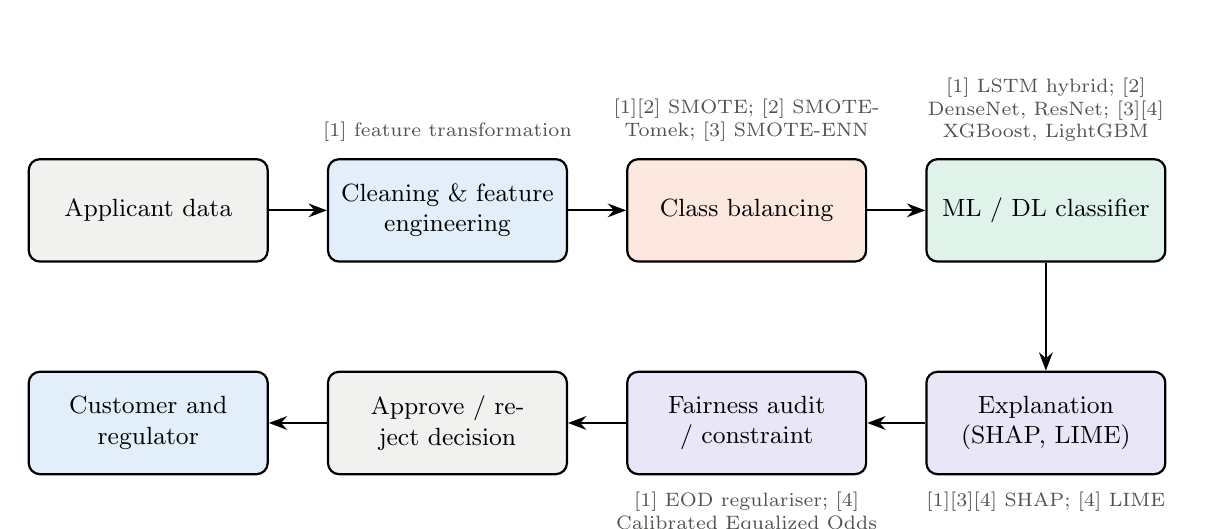
\begin{tikzpicture}[>=Stealth, thick,
  stage/.style={draw, rounded corners=4pt, align=center, text width=2.8cm, minimum height=1.3cm, font=\small},
  tag/.style={font=\scriptsize, text=inkgray, align=center, text width=3.4cm}]
\node[stage, fill=boxgray]   (d) at (0,0)     {Applicant data};
\node[stage, fill=boxblue]   (p) at (3.8,0)   {Cleaning \& feature engineering};
\node[stage, fill=boxorange] (b) at (7.6,0)   {Class balancing};
\node[stage, fill=boxgreen]  (m) at (11.4,0)  {ML / DL classifier};
\node[stage, fill=boxviolet] (x) at (11.4,-2.7) {Explanation (SHAP, LIME)};
\node[stage, fill=boxviolet] (f) at (7.6,-2.7)  {Fairness audit / constraint};
\node[stage, fill=boxgray]   (o) at (3.8,-2.7)  {Approve / reject decision};
\node[stage, fill=boxblue]   (r) at (0,-2.7)    {Customer and regulator};
\draw[->] (d) -- (p); \draw[->] (p) -- (b); \draw[->] (b) -- (m);
\draw[->] (m) -- (x); \draw[->] (x) -- (f); \draw[->] (f) -- (o); \draw[->] (o) -- (r);
\node[tag, anchor=south] at (3.8,0.75)  {[1] feature transformation};
\node[tag, anchor=south] at (7.6,0.75)  {[1][2] SMOTE; [2] SMOTE-Tomek; [3] SMOTE-ENN};
\node[tag, anchor=south] at (11.4,0.75) {[1] LSTM hybrid; [2] DenseNet, ResNet; [3][4] XGBoost, LightGBM};
\node[tag, anchor=north] at (11.4,-3.45) {[1][3][4] SHAP; [4] LIME};
\node[tag, anchor=north] at (7.6,-3.45)  {[1] EOD regulariser; [4] Calibrated Equalized Odds};
\end{tikzpicture}
\caption{A modern credit risk assessment pipeline and the stages addressed by the reviewed papers}
\label{fig:pipeline}
\end{figure}

\section{Motivation}

\paragraph{} The motivation for this seminar is the observation that high accuracy alone is no longer sufficient for credit risk models. A model that achieves excellent accuracy on a benchmark may still be unusable if it cannot explain its decisions to a rejected applicant, if it systematically disadvantages a demographic group, or if it simply predicts ``no default'' for everyone because defaults are rare. The four reviewed papers each tackle a different part of this problem, and studying them together clarifies how accuracy, imbalance handling, interpretability, and fairness interact.

\paragraph{} A second motivation is practical. Financial institutions must choose among a bewildering variety of algorithms---logistic regression, random forests, gradient-boosted trees, and many deep architectures---and among many preprocessing options. Paper \cite{p2} alone compares sixteen models under five data-balancing configurations. Understanding which families perform best on which kinds of data, and at what cost in transparency and computation, is directly useful for designing real lending systems.

\paragraph{} Finally, the topic has strong societal relevance. Access to credit shapes people's ability to study, start businesses, and own homes. Automated credit decisions that are opaque or biased can deny these opportunities unfairly, while transparent and fair models can extend credit responsibly to underserved groups, including applicants with limited credit histories.

\section{Problem Statement}

\paragraph{} \emph{Given historical data on loan applicants and their repayment outcomes, build a model that predicts default risk accurately, remains reliable when defaulters are rare, explains each decision, and does not treat applicants unfairly on the basis of sensitive attributes.}

\section{Objectives}

\paragraph{} The objectives of this seminar are:
\begin{itemize}
  \item To introduce the fundamentals of credit scoring as a supervised classification problem and the ML, ensemble, and DL techniques used to solve it.
  \item To explain the class-imbalance problem and the resampling techniques---SMOTE, SMOTE-Tomek, and SMOTE-ENN---used to address it.
  \item To present the principles of explainable AI (SHAP, LIME, surrogate models) and of fairness in machine learning (disparate impact, equal opportunity, equalized odds, intersectional fairness).
  \item To review in depth four recent IEEE papers on deep learning, ensemble learning, explainability, and fairness for credit risk and loan approval, including their methods and quantitative results.
  \item To compare the approaches and identify open challenges and future research directions for trustworthy financial risk prediction.
\end{itemize}

\section{Scope}

\paragraph{} This seminar focuses on binary credit risk and loan approval prediction from applicant-level data, as studied in papers \cite{p1}, \cite{p2}, \cite{p3}, and \cite{p4}. It covers the German Credit, Australian Credit Approval, Give Me Some Credit, CreditRisk, and bank-customer loan datasets used in these works, the evaluation metrics they report (accuracy, precision, recall, specificity, F1-score, AUC, MCC, and fairness metrics), and the XAI and fairness techniques they apply. House price prediction is discussed only as the second application domain of paper \cite{p4}. Credit card fraud detection, portfolio-level risk modelling, and macro-economic stress testing are outside the scope of this report.

\section{Advantages}

\paragraph{} Interpretable and fairness-aware ML/DL models offer several advantages over traditional credit assessment:
\begin{itemize}
  \item \textbf{Higher Accuracy:} Ensemble and deep models capture non-linear relationships and feature interactions that linear scorecards miss.
  \item \textbf{Speed and Scalability:} Automated models can assess thousands of applications in seconds, reducing processing time and operational cost.
  \item \textbf{Better Detection of Defaulters:} Resampling techniques such as SMOTE-ENN substantially improve recall and specificity on the minority (default) class.
  \item \textbf{Transparency:} SHAP and LIME explain which features drove each decision, supporting customer communication and regulatory review.
  \item \textbf{Fairness:} Fairness metrics and constraints reduce disparities in outcomes between demographic groups.
  \item \textbf{Richer Data Use:} Deep architectures can integrate structured financial records with sequential behavioural and transaction data.
  \item \textbf{Adaptability:} Models can be retrained as economic conditions and customer behaviour change.
  \item \textbf{Regulatory Alignment:} Explainable and fair models help institutions comply with data-protection and fair-lending requirements.
\end{itemize}

\section{Organization of the Report}

\paragraph{} \textbf{Chapter 2} introduces the theoretical foundations. \textbf{Chapter 3} reviews the four papers in detail. \textbf{Chapter 4} compares the approaches, \textbf{Chapter 5} discusses applications, \textbf{Chapter 6} presents challenges and future directions, and \textbf{Chapter 7} concludes the report.

% ================= CHAPTER 2: THEORETICAL FOUNDATIONS =================
\chapter{Theoretical Foundations}

\paragraph{} This chapter introduces the concepts on which the reviewed papers build: the formulation of credit scoring as a classification problem, the classical, ensemble, and deep learning models used to solve it, techniques for handling class imbalance, methods for explaining model predictions, definitions of fairness, and the metrics used for evaluation.

\section{Credit Scoring as a Classification Problem}

\paragraph{} Let $X\in\mathbb{R}^{d}$ be the feature vector describing a loan applicant---demographic attributes, income, credit history, loan characteristics, and possibly behavioural features---and let $y\in\{0,1\}$ indicate whether the applicant defaults ($y=1$) or repays ($y=0$). Given a dataset $\mathcal{D}=\{(X_i,y_i)\}_{i=1}^{n}$, the goal is to learn a function $f:\mathbb{R}^{d}\rightarrow[0,1]$ that estimates the probability of default \cite{p1}:
\begin{equation}
\hat{P}(y=1\mid X)=f(X;\theta),
\end{equation}
where $\theta$ are the model parameters. The parameters are typically learned by minimising the binary cross-entropy (BCE) loss
\begin{equation}
\mathcal{L}(\theta)=-\frac{1}{n}\sum_{i=1}^{n}\Big[y_i\log f(X_i;\theta)+(1-y_i)\log\big(1-f(X_i;\theta)\big)\Big],
\label{eq:bce}
\end{equation}
and a decision is made by comparing the predicted probability with a threshold $t$ (commonly $t=0.5$). To reduce overfitting, a penalty such as $\lambda\|\theta\|_2^2$ (L2, ridge) or $\lambda\|\theta\|_1$ (L1, lasso) is often added. The L1 penalty drives many weights to exactly zero, producing sparse and therefore more interpretable models.

\paragraph{} Two kinds of error have very different costs in lending \cite{p2}. A \textbf{false negative} (predicting ``no default'' for an applicant who defaults) causes a direct credit loss, while a \textbf{false positive} (predicting ``default'' for a creditworthy applicant) causes a lost customer and lost interest income. Because defaulters are rare, a model can reach high accuracy while missing most of them, which is why recall, specificity, F1-score, and AUC are reported alongside accuracy.

\section{Classical Machine Learning Classifiers}

\paragraph{} \textbf{Logistic Regression} models the log-odds of default as a linear function of the features \cite{p3}:
\begin{equation}
\log\frac{P}{1-P}=\beta_0+\beta_1X_1+\beta_2X_2+\cdots+\beta_kX_k .
\end{equation}
Its coefficients have a direct interpretation, which is why it remains the industry benchmark. \textbf{Decision trees} such as CART recursively split the data using the feature and threshold that most reduce impurity; for classification the Gini impurity of a node $D$ with $m$ classes is
\begin{equation}
\mathrm{Gini}(D)=1-\sum_{i=1}^{m}p_i^{2},
\end{equation}
where $p_i$ is the proportion of class $i$ in $D$. Trees yield human-readable if--then rules but are unstable and prone to overfitting. \textbf{Gaussian Naive Bayes} applies Bayes' theorem assuming conditionally independent, normally distributed features, and \textbf{K-Nearest Neighbours} (KNN) classifies an applicant by majority vote among the $k$ most similar training applicants \cite{p2}.

\section{Ensemble Learning}

\paragraph{} Ensemble methods combine many weak learners, usually decision trees, into a strong learner. \textbf{Bagging}-based \textbf{Random Forest} \cite{breiman2001} trains each tree on a bootstrap sample and considers a random subset of about $\sqrt{m}$ features at each split, then predicts by majority vote \cite{p3}:
\begin{equation}
H(x)=\operatorname{mode}\{h(x,T_1),h(x,T_2),\ldots,h(x,T_n)\}.
\end{equation}
\textbf{Boosting} instead trains learners sequentially, each focusing on the errors of its predecessors. \textbf{AdaBoost} re-weights misclassified samples and combines the weak learners as $F(x)=\sum_{t=1}^{T}\alpha_t h_t(x)$. \textbf{Gradient boosting} fits each new tree to the negative gradient of the loss. \textbf{XGBoost} \cite{chen2016} adds a regularisation term $\Omega$ that penalises tree complexity:
\begin{equation}
\mathcal{L}(\phi)=\sum_{i} l(\hat{y}_i,y_i)+\sum_{k}\Omega(f_k),
\end{equation}
and uses second-order gradient information, sparsity-aware split finding, and efficient parallel computation. \textbf{LightGBM} \cite{ke2017} grows trees leaf-wise rather than level-wise and introduces Gradient-based One-Side Sampling (GOSS), which keeps instances with large gradients, and Exclusive Feature Bundling (EFB), which merges mutually exclusive sparse features, making it very fast on large datasets \cite{p3}. Gradient-boosted trees are widely regarded as the strongest models for tabular data such as credit applications.

\section{Deep Learning Architectures}

\paragraph{} A \textbf{Multi-Layer Perceptron} (MLP) stacks fully connected layers with non-linear activations, e.g.\ $\hat{y}=\sigma\big(W_2\,\sigma(W_1x+b_1)+b_2\big)$, and is trained by back-propagation \cite{p3}. \textbf{Convolutional Neural Networks} (CNNs) apply shared filters that detect local patterns; applied to tabular data, they capture interactions between neighbouring features. \textbf{Recurrent networks} process sequences; the \textbf{Long Short-Term Memory} (LSTM) cell \cite{hochreiter1997} uses input, forget, and output gates to retain information over long sequences, which suits monthly repayment and transaction histories:
\begin{align}
f_t &= \sigma(W_f[h_{t-1},x_t]+b_f), \quad i_t=\sigma(W_i[h_{t-1},x_t]+b_i), \quad o_t=\sigma(W_o[h_{t-1},x_t]+b_o),\\
c_t &= f_t\odot c_{t-1}+i_t\odot\tanh(W_c[h_{t-1},x_t]+b_c), \qquad h_t=o_t\odot\tanh(c_t).
\end{align}
The \textbf{Gated Recurrent Unit} (GRU) is a lighter variant with two gates. \textbf{Transformers} replace recurrence with self-attention, $\mathrm{Attention}(Q,K,V)=\mathrm{softmax}(QK^{\top}/\sqrt{d_k})V$, which relates every element of a sequence to every other element. \textbf{Residual Networks} (ResNet) add skip connections, $y=\mathcal{F}(x)+x$, that make very deep networks trainable by easing gradient flow, while \textbf{DenseNet} connects each layer to all preceding layers, encouraging feature reuse with relatively few parameters \cite{p2}. \textbf{Autoencoders} learn compressed representations by reconstructing their input and are used for dimensionality reduction and anomaly detection.

\section{Handling Class Imbalance}

\paragraph{} In credit datasets the default class is typically a small minority---about 30\% of the German Credit dataset is labelled ``bad'' \cite{p3}---so classifiers are biased toward predicting the majority class. Three families of remedies are common:
\begin{itemize}
  \item \textbf{Oversampling:} the \textbf{Synthetic Minority Over-sampling Technique} (SMOTE) \cite{chawla2002} creates new minority samples by interpolating between a minority sample $x_i$ and one of its $k$ nearest minority neighbours $x_{nn}$:
  \begin{equation}
  x_{\mathrm{new}}=x_i+\lambda\,(x_{nn}-x_i),\qquad \lambda\sim U(0,1).
  \label{eq:smote}
  \end{equation}
  \item \textbf{Undersampling and cleaning:} \textbf{Tomek links} remove pairs of opposite-class nearest neighbours that lie on the class boundary, and \textbf{Edited Nearest Neighbours} (ENN) removes samples whose class disagrees with the majority of their $k$ nearest neighbours. The hybrids \textbf{SMOTE-Tomek} and \textbf{SMOTE-ENN} first oversample and then clean noisy and overlapping samples.
  \item \textbf{Cost-sensitive learning:} class weights $w_{y_i}$ increase the loss for misclassifying minority samples, $\mathcal{L}_{\mathrm{weighted}}=-\frac{1}{n}\sum_i w_{y_i}[y_i\log\hat{y}_i+(1-y_i)\log(1-\hat{y}_i)]$; focal loss further down-weights easy examples \cite{p1}.
\end{itemize}
Figure~\ref{fig:smote} illustrates SMOTE interpolation and ENN cleaning. Resampling must be applied only to the training set; applying it before the train/test split would leak synthetic information into the evaluation.

\begin{figure}[htbp]
\centering
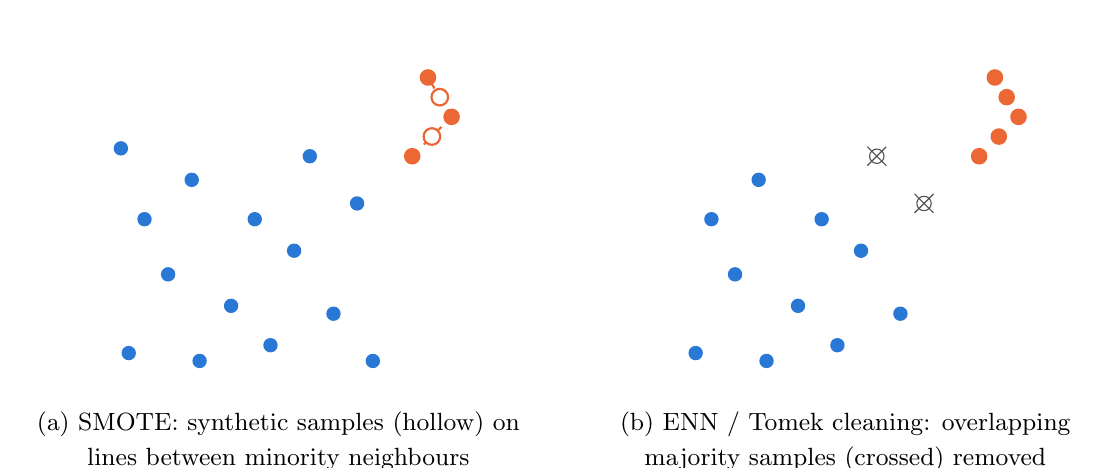
\begin{tikzpicture}[>=Stealth]
\begin{scope}
\foreach \x/\y in {0.3/0.4,0.8/1.4,1.2/0.3,1.6/1.0,2.1/0.5,0.5/2.1,2.4/1.7,1.1/2.6,2.9/0.9,3.2/2.3,2.6/2.9,0.2/3.0,3.4/0.3,1.9/2.1}
  \fill[seriesA] (\x,\y) circle (2.6pt);
\foreach \x/\y in {3.9/2.9,4.4/3.4,4.1/3.9}
  \fill[seriesB] (\x,\y) circle (3pt);
\draw[seriesB, thick, dashed] (3.9,2.9) -- (4.4,3.4);
\draw[seriesB, thick, dashed] (4.4,3.4) -- (4.1,3.9);
\filldraw[fill=white, draw=seriesB, thick] (4.15,3.15) circle (3pt);
\filldraw[fill=white, draw=seriesB, thick] (4.25,3.65) circle (3pt);
\node[font=\small] at (2.2,-0.5) {(a) SMOTE: synthetic samples (hollow) on};
\node[font=\small] at (2.2,-0.95) {lines between minority neighbours};
\end{scope}
\begin{scope}[xshift=7.2cm]
\foreach \x/\y in {0.3/0.4,0.8/1.4,1.2/0.3,1.6/1.0,2.1/0.5,0.5/2.1,2.4/1.7,1.1/2.6,2.9/0.9,1.9/2.1}
  \fill[seriesA] (\x,\y) circle (2.6pt);
\foreach \x/\y in {3.2/2.3,2.6/2.9}
  {\draw[inkgray] (\x,\y) circle (2.6pt); \draw[inkgray] (\x-0.12,\y-0.12) -- (\x+0.12,\y+0.12); \draw[inkgray] (\x-0.12,\y+0.12) -- (\x+0.12,\y-0.12);}
\foreach \x/\y in {3.9/2.9,4.4/3.4,4.1/3.9,4.15/3.15,4.25/3.65}
  \fill[seriesB] (\x,\y) circle (3pt);
\node[font=\small] at (2.2,-0.5) {(b) ENN / Tomek cleaning: overlapping};
\node[font=\small] at (2.2,-0.95) {majority samples (crossed) removed};
\end{scope}
\end{tikzpicture}
\caption{Illustration of hybrid resampling. Blue: majority (non-default) class; orange: minority (default) class.}
\label{fig:smote}
\end{figure}

\section{Explainable Artificial Intelligence}

\paragraph{} Explainable AI methods make the behaviour of complex models understandable to humans. \textbf{Global} explanations describe which features matter across the whole dataset, while \textbf{local} explanations describe why a specific applicant received a specific decision.

\paragraph{} \textbf{SHAP} (SHapley Additive exPlanations) \cite{lundberg2017} assigns each feature a contribution based on the Shapley value from cooperative game theory---the average marginal contribution of the feature across all possible subsets (coalitions) of the other features \cite{p3}:
\begin{equation}
\phi_j=\sum_{S\subseteq F\setminus\{j\}}\frac{|S|!\,(|F|-|S|-1)!}{|F|!}\Big[f_{S\cup\{j\}}(x_{S\cup\{j\}})-f_S(x_S)\Big],
\label{eq:shap}
\end{equation}
where $F$ is the set of all features. SHAP values are additive: the base value plus the sum of all $\phi_j$ equals the model output for that applicant. Summary plots rank features by the mean absolute SHAP value, $\mathrm{Importance}_j=\frac{1}{n}\sum_i|\phi_j^{(i)}|$, and force plots explain individual predictions. Efficient exact algorithms exist for tree ensembles.

\paragraph{} \textbf{LIME} (Local Interpretable Model-agnostic Explanations) \cite{ribeiro2016} explains a single prediction by fitting a simple interpretable model $g$ (e.g.\ a sparse linear model) to the black-box model $f$ in the neighbourhood of the instance $x$:
\begin{equation}
\xi(x)=\arg\min_{g\in G}\;\mathcal{L}(f,g,\pi_x)+\Omega(g),
\end{equation}
where $\pi_x$ weights perturbed samples by their proximity to $x$ and $\Omega(g)$ penalises complexity. Other tools include \textbf{Partial Dependence Plots} (PDPs) and \textbf{Accumulated Local Effects} (ALE), which show how the prediction changes with a feature, and \textbf{surrogate models}, such as a decision tree trained to mimic a deep network's predictions \cite{p1,p4}.

\section{Fairness in Machine Learning}

\paragraph{} Let $A$ denote a sensitive attribute (e.g.\ gender or age group) and $\hat{Y}$ the model's decision. Common group fairness criteria are:
\begin{itemize}
  \item \textbf{Demographic parity / Disparate Impact (DI):} positive decisions should be equally likely across groups; $\mathrm{DI}=P(\hat{Y}=1\mid A=a)/P(\hat{Y}=1\mid A=b)$, with values near 1 indicating parity.
  \item \textbf{Equal opportunity:} true positive rates should be equal across groups; the \textbf{Equal Opportunity Difference} is $\mathrm{EOD}=|\mathrm{TPR}_{A=a}-\mathrm{TPR}_{A=b}|$ \cite{p1}.
  \item \textbf{Equalized odds:} both true positive and false positive rates should be equal across groups. \textbf{Calibrated Equalized Odds} post-processes the scores of a calibrated classifier to reduce these disparities while preserving calibration \cite{p4}.
  \item \textbf{Intersectional fairness:} fairness is evaluated for combinations of attributes (e.g.\ gender $\times$ income), since a model can appear fair on each attribute separately while disadvantaging a specific intersection.
\end{itemize}
Bias mitigation can be applied before training (re-weighting or resampling data), during training (fairness regularisers or adversarial debiasing), or after training (adjusting thresholds or scores). Different fairness criteria can conflict with each other and with accuracy, so the choice of criterion is itself a policy decision.

\section{Evaluation Metrics}

\paragraph{} Most metrics are derived from the confusion matrix of true positives (TP), true negatives (TN), false positives (FP), and false negatives (FN) \cite{p2,p3}. Table~\ref{tab:metrics} lists the definitions used in the reviewed papers. The \textbf{AUC} is the area under the ROC curve, which plots the true positive rate against the false positive rate across all decision thresholds; an AUC of 1 indicates perfect separation and 0.5 indicates random guessing. The \textbf{Matthews Correlation Coefficient} (MCC) ranges from $-1$ to $+1$ and remains informative even when classes are highly imbalanced, which makes it a useful complement to accuracy. Fairness is evaluated with DI and EOD as defined in the previous section.

{\renewcommand{\arraystretch}{1.6}
\begin{table}[htbp]
\centering
\caption{Evaluation metrics used in the reviewed papers}\label{tab:metrics}
\small
\begin{tabularx}{\textwidth}{|p{2.0cm}|p{8.0cm}|X|}
\hline
\textbf{Metric} & \textbf{Definition} & \textbf{Interpretation} \\ \hline
Accuracy & $\dfrac{TP+TN}{TP+TN+FP+FN}$ & Overall fraction of correct decisions \\ \hline
Precision & $\dfrac{TP}{TP+FP}$ & Reliability of positive predictions \\ \hline
Recall (TPR) & $\dfrac{TP}{TP+FN}$ & Fraction of actual positives detected \\ \hline
Specificity & $\dfrac{TN}{TN+FP}$ & Fraction of actual negatives detected \\ \hline
F1-score & $\dfrac{2\cdot\mathrm{Precision}\cdot\mathrm{Recall}}{\mathrm{Precision}+\mathrm{Recall}}$ & Balance of precision and recall \\ \hline
MCC & $\dfrac{TP\cdot TN-FP\cdot FN}{\sqrt{(TP{+}FP)(TP{+}FN)(TN{+}FP)(TN{+}FN)}}$ & Correlation between predictions and labels \\ \hline
AUC & Area under the ROC curve & Ranking quality across thresholds \\ \hline
\end{tabularx}
\end{table}}

\section{Taxonomy of Approaches}

\paragraph{} The techniques above can be organised into a taxonomy of trustworthy credit risk modelling, shown in Figure~\ref{fig:taxonomy}. The four reviewed papers occupy different branches: \cite{p1} and \cite{p2} emphasise deep learning, \cite{p2} and \cite{p3} emphasise ensembles and resampling, \cite{p3} and \cite{p4} emphasise post-hoc explanation, and \cite{p1} and \cite{p4} address fairness explicitly.

\begin{figure}[htbp]
\centering
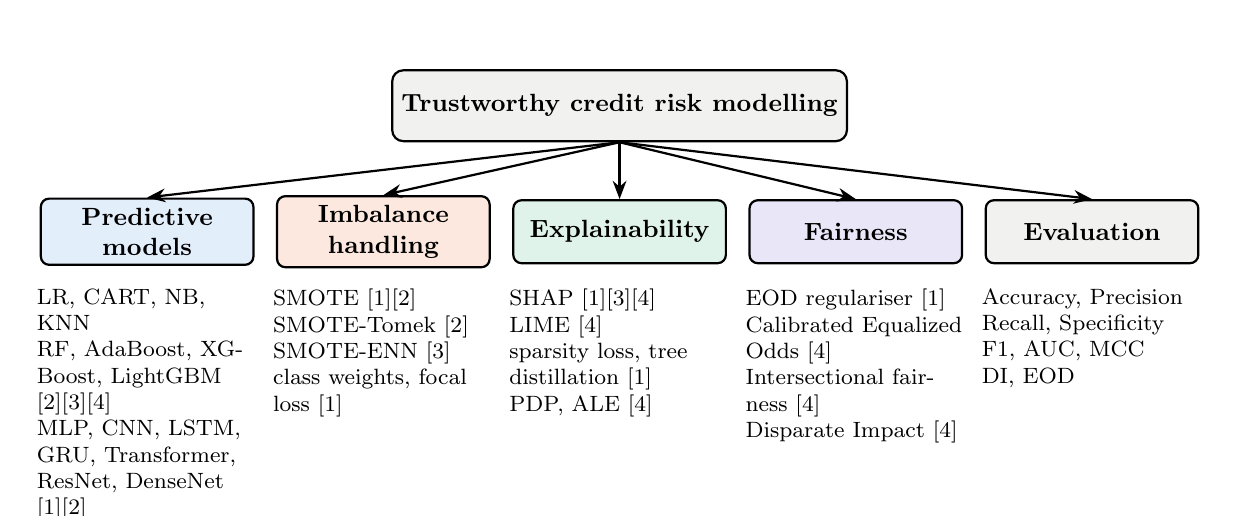
\begin{tikzpicture}[>=Stealth, thick,
  root/.style={draw, rounded corners=4pt, fill=boxgray, font=\small\bfseries, minimum width=5.2cm, minimum height=0.9cm, align=center},
  cat/.style={draw, rounded corners=3pt, font=\small\bfseries, minimum width=2.7cm, minimum height=0.8cm, align=center},
  leaf/.style={font=\footnotesize, align=left, text width=2.8cm}]
\node[root] (r) at (6.3,0) {Trustworthy credit risk modelling};
\node[cat, fill=boxblue]   (c1) at (0.3,-1.6) {Predictive\\models};
\node[cat, fill=boxorange] (c2) at (3.3,-1.6) {Imbalance\\handling};
\node[cat, fill=boxgreen]  (c3) at (6.3,-1.6) {Explainability};
\node[cat, fill=boxviolet] (c4) at (9.3,-1.6) {Fairness};
\node[cat, fill=boxgray]   (c5) at (12.3,-1.6) {Evaluation};
\foreach \c in {c1,c2,c3,c4,c5} \draw[->] (r.south) -- (\c.north);
\node[leaf, anchor=north] at (0.3,-2.2) {LR, CART, NB, KNN\\RF, AdaBoost, XGBoost, LightGBM [2][3][4]\\MLP, CNN, LSTM, GRU, Transformer, ResNet, DenseNet [1][2]};
\node[leaf, anchor=north] at (3.3,-2.2) {SMOTE [1][2]\\SMOTE-Tomek [2]\\SMOTE-ENN [3]\\class weights, focal loss [1]};
\node[leaf, anchor=north] at (6.3,-2.2) {SHAP [1][3][4]\\LIME [4]\\sparsity loss, tree distillation [1]\\PDP, ALE [4]};
\node[leaf, anchor=north] at (9.3,-2.2) {EOD regulariser [1]\\Calibrated Equalized Odds [4]\\Intersectional fairness [4]\\Disparate Impact [4]};
\node[leaf, anchor=north] at (12.3,-2.2) {Accuracy, Precision\\Recall, Specificity\\F1, AUC, MCC\\DI, EOD};
\end{tikzpicture}
\caption{Taxonomy of techniques for trustworthy credit risk modelling and the papers that use them}
\label{fig:taxonomy}
\end{figure}

\section{Regulatory and Ethical Context}

\paragraph{} Credit scoring is one of the most heavily regulated applications of machine learning. In the European Union, the GDPR restricts decisions based solely on automated processing that significantly affect individuals and requires that they receive meaningful information about the logic involved, and the EU Artificial Intelligence Act classifies AI systems used to evaluate the creditworthiness of natural persons as \emph{high-risk}, subjecting them to requirements on data quality, documentation, transparency, and human oversight. In the United States, fair-lending law requires lenders to give applicants the principal reasons for an adverse credit decision and prohibits discrimination on protected characteristics. Banking supervisors also expect institutions to validate their risk models and to understand their limitations.

\paragraph{} These requirements translate directly into the technical themes of this report: explanations are needed to state reasons for decisions, fairness metrics are needed to demonstrate non-discrimination, and robust evaluation on imbalanced data is needed for sound model validation. The reviewed papers explicitly connect their XAI and fairness components to such requirements \cite{p1,p4}.

\section{Chapter Summary}

\paragraph{} This chapter formulated credit scoring as binary classification and introduced the models used in the reviewed papers, from logistic regression and decision trees to gradient-boosted ensembles and deep networks such as LSTM, ResNet, and DenseNet. It explained why class imbalance distorts both training and evaluation, and how SMOTE, SMOTE-Tomek, SMOTE-ENN, and cost-sensitive losses correct it. It then introduced SHAP and LIME for explanation, group fairness criteria for auditing, and the evaluation metrics used in the next chapter.


% -----------------------------
% CHAPTER 3: LITERATURE SURVEY
% -----------------------------
\chapter{Literature Survey}

\paragraph{} This chapter reviews the four selected IEEE Access papers on interpretable and fair machine learning for credit risk and loan approval. For each paper, the problem addressed, the proposed methodology with its key equations, the experimental setup, and the principal results are presented, followed by a brief critical discussion.

%---------------------------------------------------------------
\section{Credit Scoring Prediction Using Deep Learning Models in the Financial Sector}

This paper by Shi, Tang, and Yu \cite{p1} proposes a unified deep learning framework for credit scoring that integrates structured financial records with unstructured behavioural data, models temporal patterns with LSTM layers, and embeds interpretability, class-imbalance handling, and fairness directly into the training objective.

\subsection{Problem Statement and Motivation}

\paragraph{} Traditional scoring systems based on static rules and historical credit behaviour cannot capture the dynamic, non-linear nature of consumer financial behaviour in the digital economy. Classical ML models improve on rules but depend on manual feature engineering and structured inputs, and struggle with temporal dependencies. Deep models capture such dependencies but are criticised as black boxes, and most prior work addresses fairness and interpretability only as post-hoc concerns. The authors therefore aim to build a framework that (i) handles heterogeneous data including transaction histories, (ii) captures temporal behaviour, (iii) is robust to class imbalance, and (iv) provides interpretability and fairness suitable for regulatory scrutiny.

\subsection{Hybrid Credit Scoring Model}

\paragraph{} The model (Figure~\ref{fig:p1_model}) consists of feature transformation, a hybrid deep architecture, and a hybrid loss function.

\paragraph{} \textbf{Feature transformation.} Continuous features such as income, loan amount, and credit score are normalised with min--max scaling, $x_{\mathrm{scaled}}=(x-\min(x))/(\max(x)-\min(x))$, so that no feature dominates due to its scale. Categorical features such as occupation or loan type are mapped to dense embedding vectors $e_i\in\mathbb{R}^{k}$ instead of sparse one-hot vectors. Dimensionality is then reduced either linearly with PCA, $V=\arg\max_V \mathrm{Var}(XV)$, or non-linearly with an autoencoder trained to minimise the reconstruction error $\|X-f_\theta(X)\|_2^2$.

\paragraph{} \textbf{Deep learning architecture.} The transformed features pass through an LSTM layer that models sequential behaviour such as monthly spending and repayment patterns, followed by fully connected ReLU layers that model non-linear feature interactions, and a sigmoid output that gives the probability of default:
\begin{equation}
\hat{y}=\sigma\Big(W_3\cdot\mathrm{ReLU}\big(W_2\cdot\mathrm{LSTM}(W_1X+b_1)+b_2\big)+b_3\Big).
\end{equation}

\paragraph{} \textbf{Hybrid loss.} To make the model focus on a small set of influential features, the binary cross-entropy is combined with an L1 sparsity term on the feature weights:
\begin{equation}
\mathcal{L}_{\mathrm{hybrid}}=\mathcal{L}_{\mathrm{binary}}+\lambda\,\mathcal{L}_{\mathrm{interpretability}},\qquad \mathcal{L}_{\mathrm{interpretability}}=\sum_{j=1}^{d}|w_j|,
\end{equation}
where $\lambda$ trades predictive accuracy against interpretability; larger $\lambda$ yields a sparser, more transparent model and also reduces overfitting.

\begin{figure}[htbp]
   \centering
   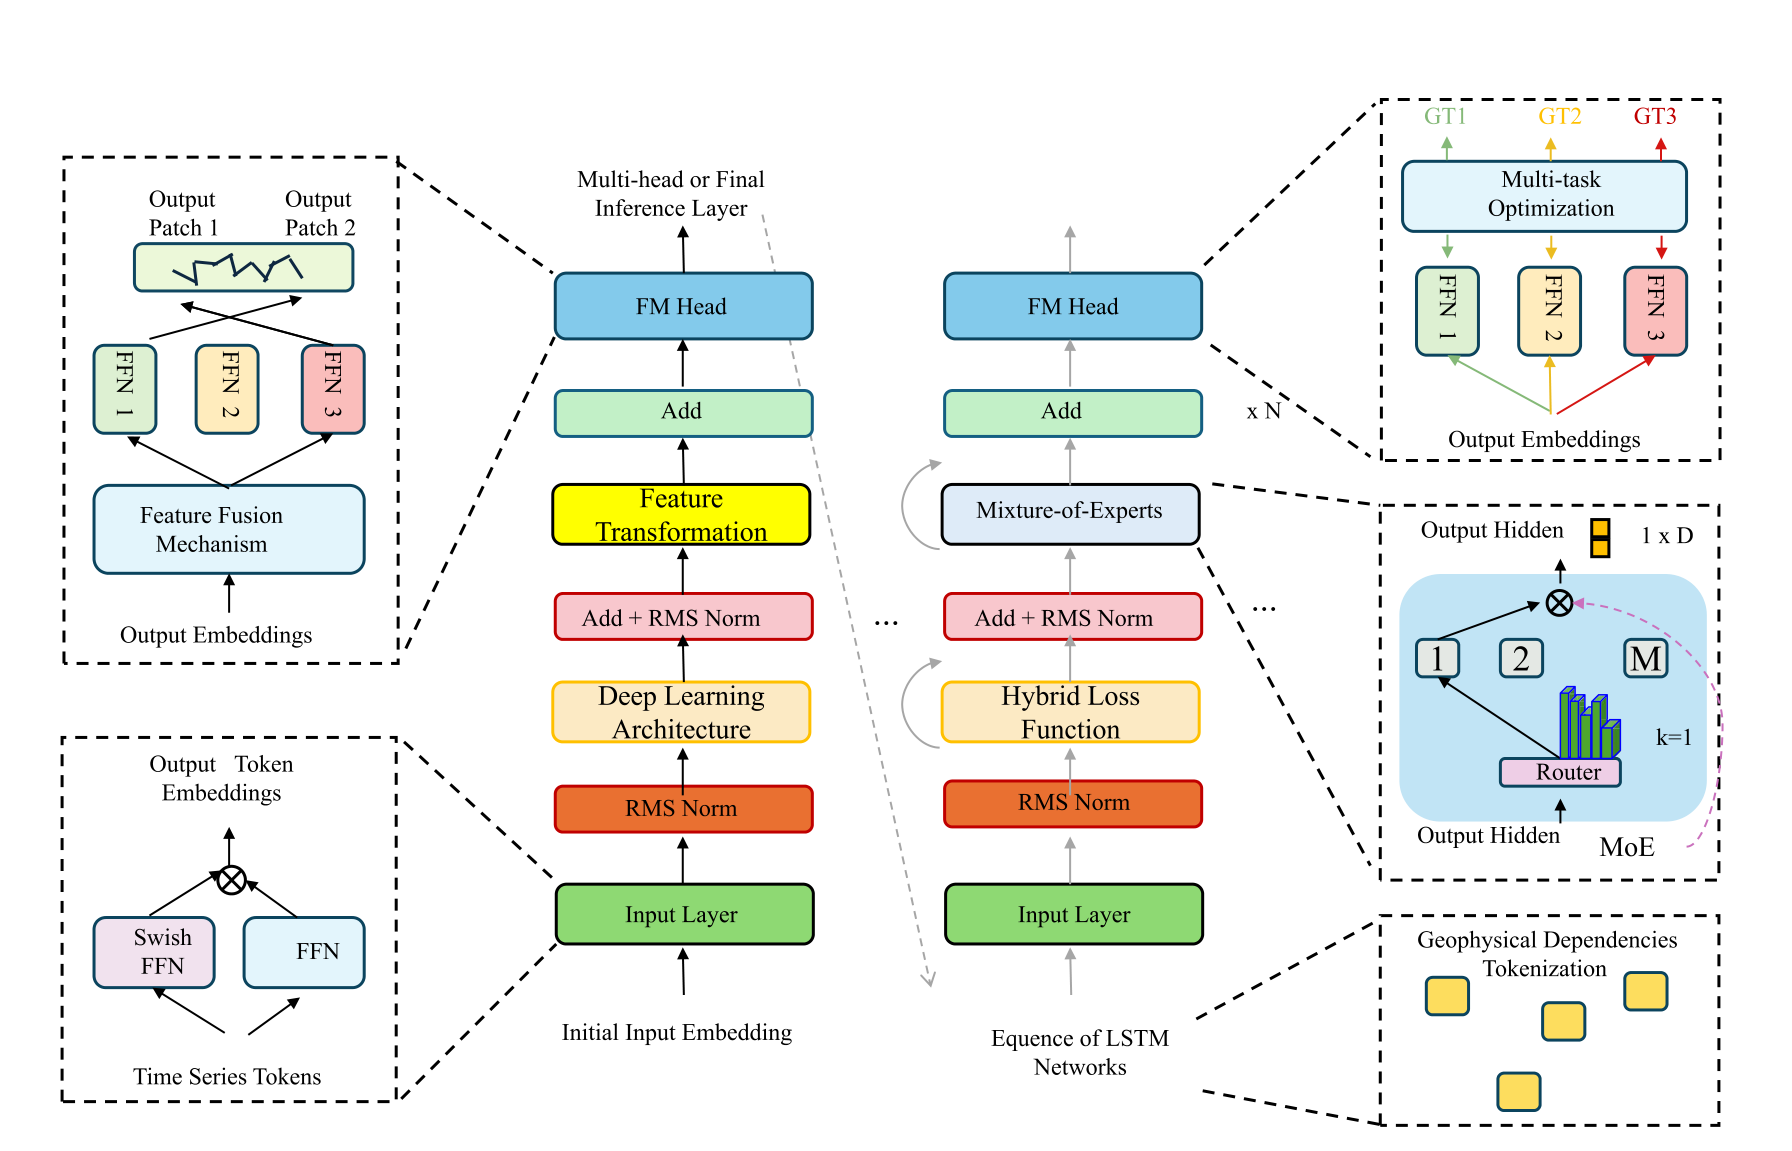
\includegraphics[width=0.85\linewidth,keepaspectratio]{figs/p1_hybrid_model.png}
   \caption{Architecture of the hybrid credit scoring model with feature transformation, LSTM-based deep architecture, and hybrid loss \cite{p1}}
   \label{fig:p1_model}
\end{figure}

\subsection{Enhanced Credit Scoring Strategy}

\paragraph{} \textbf{Feature engineering.} Traditional financial features (income, credit history, debt) are combined with behavioural features derived from transactions---average monthly spending, repayment frequency, time gaps between payments, and variability of transaction amounts. Interaction terms $x_{\mathrm{interaction}}=x_i\cdot x_j$ capture combined effects such as that of income and debt together.

\paragraph{} \textbf{Adaptive regularisation.} In addition to L2 regularisation $\lambda\sum_j w_j^2$, the authors propose an adaptive penalty proportional to the ratio of validation to training loss, $\mathcal{L}_{\mathrm{adaptive}}=\alpha\,\mathcal{L}_{\mathrm{val}}/\mathcal{L}_{\mathrm{train}}$, which increases regularisation when the model begins to overfit and relaxes it when it underfits.

\paragraph{} \textbf{Imbalance handling.} SMOTE (Equation~\ref{eq:smote}) generates synthetic defaulters, a class-weighted cross-entropy increases the penalty for misclassifying defaulters, and \emph{hard example mining} focuses training on samples near the decision boundary. Focal loss is also used on the CreditRisk dataset.

\paragraph{} \textbf{Model transparency.} SHAP values (Equation~\ref{eq:shap}) quantify each feature's contribution, and global importance is computed as the mean absolute SHAP value. A decision tree is additionally trained by \emph{model distillation} to mimic the deep model, minimising $\mathcal{L}_{\mathrm{tree}}=\sum_i(\hat{y}_i-\hat{y}^{\mathrm{tree}}_i)^2$, so that the network's behaviour can be summarised as readable if--then rules. Finally, a fairness-aware regulariser penalises differences in performance between demographic groups, measured by the Equal Opportunity Difference. Figure~\ref{fig:p1_strategy} shows the overall workflow.

\begin{figure}[htbp]
   \centering
   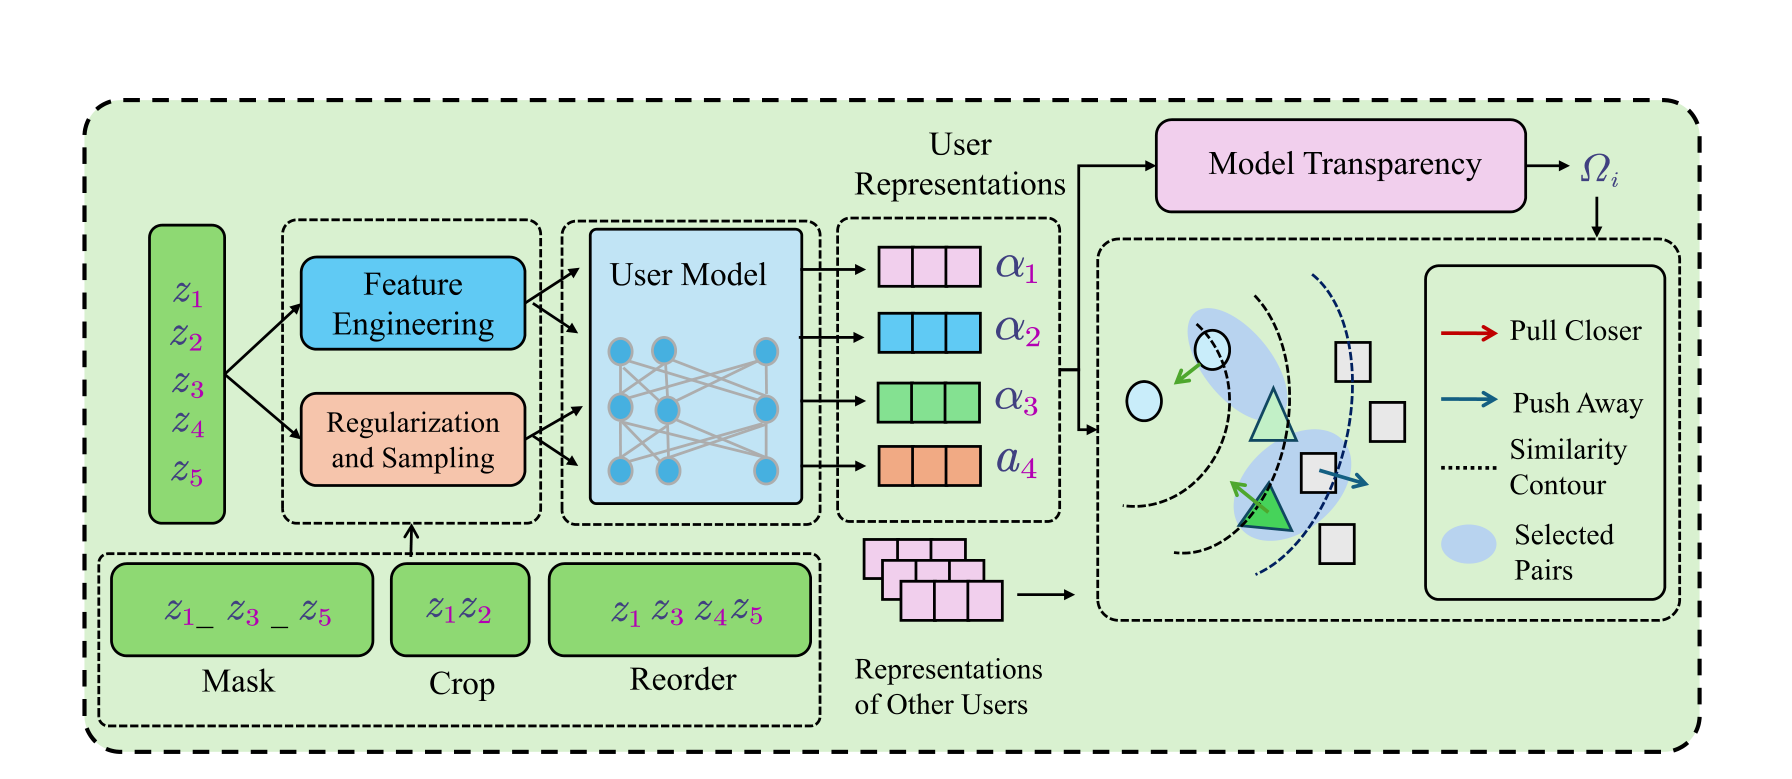
\includegraphics[width=0.85\linewidth,keepaspectratio]{figs/p1_strategy.png}
   \caption{Workflow of the enhanced credit scoring strategy: feature engineering, regularisation and sampling, user representations, and model transparency \cite{p1}}
   \label{fig:p1_strategy}
\end{figure}

\subsection{Experimental Setup}

\paragraph{} The model is evaluated on four text-classification benchmarks (THUCNews, SciHTC, UTCD) and CreditRisk to test generalisation, and on two credit-scoring datasets: \textbf{German Credit} (1{,}000 applicants labelled good or bad) and \textbf{Give Me Some Credit} (over 150{,}000 records with delinquency and credit-usage variables). Table~\ref{tab:p1_setup} lists the main implementation details.

{\renewcommand{\arraystretch}{1.2}
\begin{table}[htbp]
\centering
\caption{Implementation details of the hybrid deep credit scoring framework \cite{p1}}\label{tab:p1_setup}
\small
\begin{tabularx}{\textwidth}{|p{4.2cm}|X|}
\hline
\textbf{Item} & \textbf{Setting} \\ \hline
Framework and hardware & PyTorch 2.1, single NVIDIA A100 (80 GB) GPU \\ \hline
Optimiser & AdamW, learning rate $2\times10^{-5}$, 10\% linear warm-up \\ \hline
Training & Up to 10 epochs with early stopping; dropout 0.1; batch size 32 \\ \hline
Data split & 80/10/10 train/validation/test; mean over three random seeds \\ \hline
Tabular preprocessing & Median imputation, one-hot encoding, normalisation \\ \hline
Imbalance handling & Focal loss and SMOTE oversampling (CreditRisk) \\ \hline
Metrics & Accuracy, Precision, F1-score, AUC; EOD for fairness \\ \hline
\end{tabularx}
\end{table}}

\subsection{Results and Analysis}

\paragraph{} \textbf{Credit scoring benchmarks.} Table~\ref{tab:p1_credit} and Figure~\ref{fig:p1_chart} compare the proposed model with logistic regression, random forest, XGBoost, and LightGBM. The model achieves the best result on every metric, with AUC of 85.30\% on German Credit and 90.56\% on Give Me Some Credit, compared with 83.07\% and 88.24\% for the strongest baseline, LightGBM. The higher F1-scores indicate better handling of class imbalance.

{\renewcommand{\arraystretch}{1.2}
\begin{table}[htbp]
\centering
\caption{Performance (\%) on credit scoring datasets \cite{p1}}\label{tab:p1_credit}
\small
\begin{tabular}{|l|c|c|c|c|c|c|c|c|}
\hline
\multirow{2}{*}{\textbf{Model}} & \multicolumn{4}{c|}{\textbf{German Credit}} & \multicolumn{4}{c|}{\textbf{Give Me Some Credit}} \\ \cline{2-9}
 & Acc. & Prec. & F1 & AUC & Acc. & Prec. & F1 & AUC \\ \hline
Logistic Regression & 76.45 & 74.20 & 75.03 & 78.41 & 81.32 & 80.11 & 80.50 & 83.25 \\ \hline
Random Forest & 78.21 & 76.67 & 77.10 & 80.93 & 83.14 & 82.32 & 82.44 & 85.60 \\ \hline
XGBoost & 79.33 & 77.44 & 78.20 & 82.15 & 85.76 & 84.11 & 84.54 & 87.90 \\ \hline
LightGBM & 80.01 & 78.32 & 78.94 & 83.07 & 86.33 & 85.02 & 85.45 & 88.24 \\ \hline
\textbf{Proposed} & \textbf{82.12} & \textbf{80.41} & \textbf{81.26} & \textbf{85.30} & \textbf{88.74} & \textbf{87.19} & \textbf{87.85} & \textbf{90.56} \\ \hline
\end{tabular}
\end{table}}

\begin{figure}[htbp]
\centering
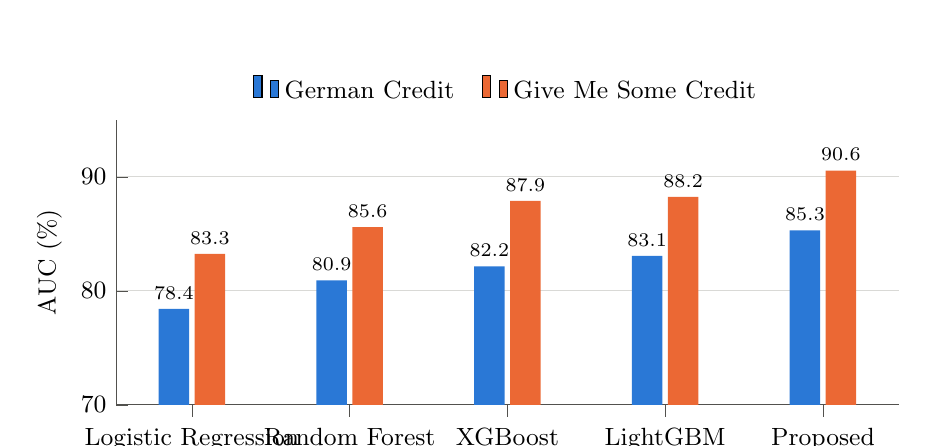
\begin{tikzpicture}
\begin{axis}[
  ybar=2pt, bar width=11pt, width=0.95\textwidth, height=5.2cm,
  symbolic x coords={Logistic Regression,Random Forest,XGBoost,LightGBM,Proposed},
  xtick=data, enlarge x limits=0.12, ymin=70, ymax=95,
  ylabel={AUC (\%)}, ylabel style={font=\small},
  ymajorgrids, grid style={gridgray}, axis line style={inkgray}, tick style={inkgray},
  axis x line*=bottom, axis y line*=left, tick label style={font=\small},
  nodes near coords, nodes near coords style={font=\scriptsize, text=black},
  every node near coord/.append style={/pgf/number format/fixed, /pgf/number format/fixed zerofill, /pgf/number format/precision=1},
  legend style={at={(0.5,1.02)}, anchor=south, legend columns=-1, draw=none, font=\small, /tikz/every even column/.append style={column sep=8pt}},
]
\addplot[fill=seriesA, draw=none] coordinates {(Logistic Regression,78.41) (Random Forest,80.93) (XGBoost,82.15) (LightGBM,83.07) (Proposed,85.30)};
\addplot[fill=seriesB, draw=none] coordinates {(Logistic Regression,83.25) (Random Forest,85.60) (XGBoost,87.90) (LightGBM,88.24) (Proposed,90.56)};
\legend{German Credit, Give Me Some Credit}
\end{axis}
\end{tikzpicture}
\caption{AUC of the proposed model and baselines on the two credit datasets, plotted from \cite{p1} (y-axis starts at 70\%)}
\label{fig:p1_chart}
\end{figure}

\paragraph{} \textbf{Comparison with text-classification models.} On the CreditRisk dataset the model also outperforms TextCNN, FastText, BiLSTM, Transformer, BERT, and RoBERTa, reaching 85.14\% accuracy, 83.56\% F1, and 88.52\% AUC against 83.49\%, 80.85\%, and 86.14\% for RoBERTa.

\paragraph{} \textbf{Ablation and fairness.} Table~\ref{tab:p1_ablation} shows the effect of adding tuning, SMOTE, and fairness regularisation step by step. Each component improves accuracy and AUC, and the Equal Opportunity Difference falls from 0.124 to 0.036, showing that fairness improves together with accuracy rather than at its expense. Removing individual modules on CreditRisk lowers F1 from 83.56\% to 77.10\% (without feature transformation), 78.09\% (without the deep architecture), and 79.35\% (without regularisation and sampling). In a demographic case study on Give Me Some Credit, F1-scores for applicants below and above age 40 were 0.882 and 0.874, with an EOD of 0.036.

{\renewcommand{\arraystretch}{1.2}
\begin{table}[htbp]
\centering
\caption{Ablation on tuning, SMOTE sampling, and fairness regularisation \cite{p1}}\label{tab:p1_ablation}
\small
\begin{tabular}{|l|c|c|c|c|}
\hline
\textbf{Configuration} & \textbf{Accuracy} & \textbf{F1} & \textbf{AUC} & \textbf{EOD} $\downarrow$ \\ \hline
Baseline (no tuning, no SMOTE, no fairness) & 85.14 & 83.07 & 87.56 & 0.124 \\ \hline
Grid search tuning only & 87.92 & 85.81 & 89.34 & 0.097 \\ \hline
Bayesian tuning only & 88.45 & 86.52 & 90.02 & 0.082 \\ \hline
+ SMOTE sampling & 89.76 & 88.14 & 91.85 & 0.068 \\ \hline
+ Fairness-aware regularisation & \textbf{90.74} & \textbf{88.93} & \textbf{92.10} & \textbf{0.036} \\ \hline
\end{tabular}
\end{table}}

\subsection{Discussion}

\paragraph{} The paper's main strength is its integrated design: temporal modelling, sparsity-based interpretability, imbalance handling, distillation into rules, and fairness regularisation are combined in one framework rather than added afterwards. Two limitations should be noted. First, much of the evaluation uses text-classification benchmarks, and only two of the datasets are credit-scoring datasets, so further validation on real bank data with behavioural sequences is needed. Second, as the authors acknowledge, the model relies on high-quality behavioural data that not all institutions possess, and its explanations remain less direct than those of a traditional scorecard; transfer learning, domain adaptation, and attention-based explanations are proposed as future work.

%---------------------------------------------------------------
\section{Machine Learning and Deep Learning for Loan Prediction in Banking: Exploring Ensemble Methods and Data Balancing}

This paper by Sayed, Alabrah, Rahouma, Zohaib, and Badry \cite{p2} presents a large comparative study of machine learning and deep learning classifiers for predicting loan defaults of bank customers, and examines how data balancing (SMOTE and SMOTE-Tomek) and ensemble methods affect their performance.

\subsection{Problem Statement and Motivation}

\paragraph{} Growing competition and the rising number of loan applications make manual eligibility checks slow and error-prone. The authors frame the problem in terms of Type I errors (rejecting a good loan, harming customer relations and revenue) and Type II errors (approving a bad loan, causing defaults and losses). They identify three gaps in the literature: under-use of ensemble methods, insufficient handling of imbalanced data, and limited attention to interpretability.

\subsection{Dataset and Proposed Architecture}

\paragraph{} The study uses a Kaggle bank dataset of \textbf{252{,}000 records and 13 features}: identifier, income, age, professional experience, marital status, house ownership, car ownership, profession, city, state, current job years, current house years, and the target \emph{Risk Flag} (defaulted on a loan). The data are split 80:20 into training and test sets. The proposed architecture (Figure~\ref{fig:p2_arch}) has two phases: data analysis and preprocessing, followed by model optimisation and classification with ML and DL models.

\begin{figure}[htbp]
   \centering
   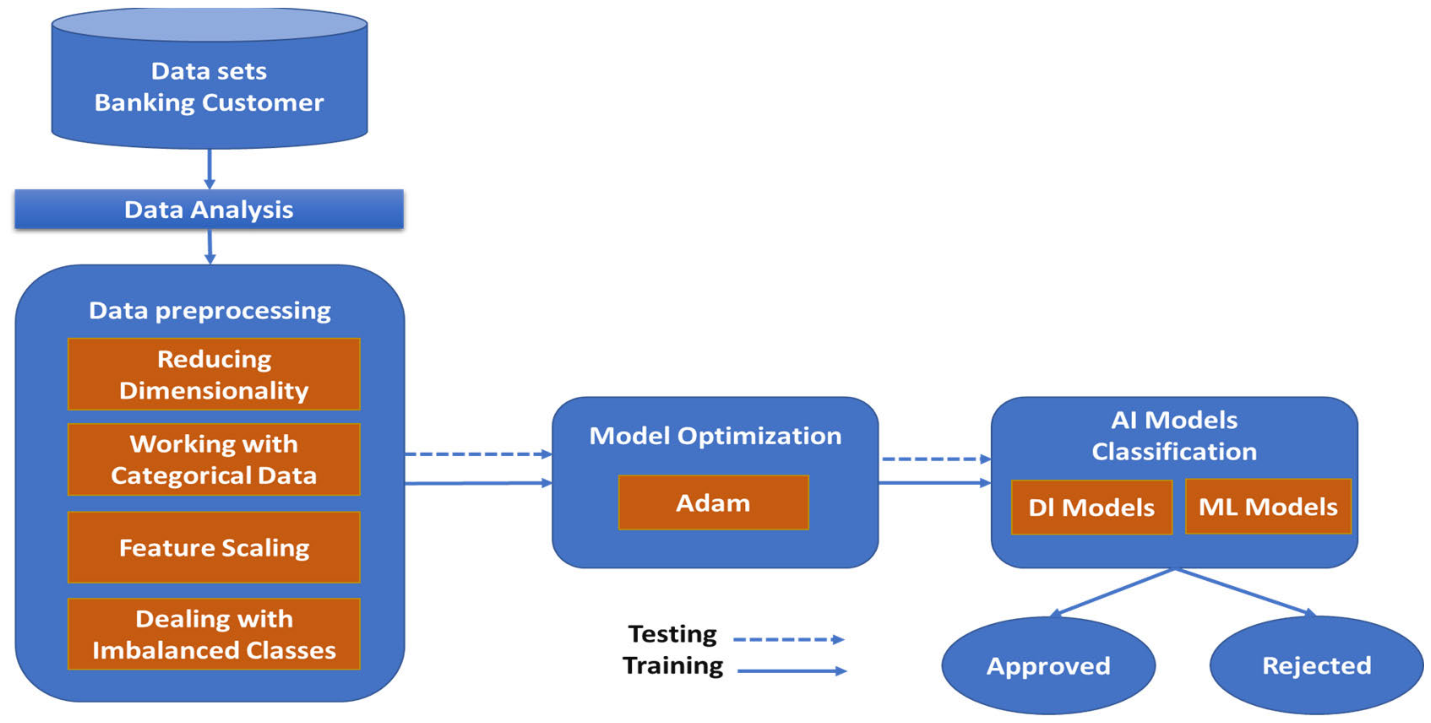
\includegraphics[width=0.72\linewidth,keepaspectratio]{figs/p2_architecture.png}
   \caption{Proposed loan prediction architecture: data analysis, preprocessing, Adam optimisation, and ML/DL classification into approved or rejected \cite{p2}}
   \label{fig:p2_arch}
\end{figure}

\subsection{Data Preprocessing and Optimisation}

\paragraph{} Preprocessing includes \textbf{dimensionality reduction} (removing the identifier column), \textbf{ordinal encoding} for ordered categories, \textbf{one-hot encoding} (``get dummies'') for nominal categories such as profession and city, \textbf{feature scaling} by standardisation, min--max scaling, or robust scaling, and \textbf{class balancing}. The target is highly imbalanced, so SMOTE oversampling and SMOTE-Tomek (SMOTE followed by removal of Tomek-link boundary pairs) are applied. Deep models are trained with the \textbf{Adam} optimiser, which adapts the learning rate of each parameter using running estimates of the first and second moments of the gradient:
\begin{equation}
m_t=\beta_1m_{t-1}+(1-\beta_1)g_t,\quad v_t=\beta_2v_{t-1}+(1-\beta_2)g_t^{2},\quad \theta_t=\theta_{t-1}-\eta\,\frac{\hat{m}_t}{\sqrt{\hat{v}_t}+\epsilon},
\end{equation}
where $\hat{m}_t$ and $\hat{v}_t$ are bias-corrected moments. Hyperparameters are tuned with grid and random search, and k-fold cross-validation and L1/L2 regularisation are used to control overfitting.

\subsection{Models}

\paragraph{} Figure~\ref{fig:p2_models} lists the models. The ML group comprises Gaussian Naive Bayes, AdaBoost, Gradient Boosting, K-Nearest Neighbours, Logistic Regression, Decision Trees, and Random Forest. The DL group comprises MLP, CNN, LSTM, Transformer, GRU, Autoencoder, ResNet, and DenseNet, with CNN-LSTM and Bidirectional LSTM also evaluated in some settings. Model performance is measured by accuracy, precision, recall, F1-score, AUC-ROC, and MCC.

\begin{figure}[htbp]
   \centering
   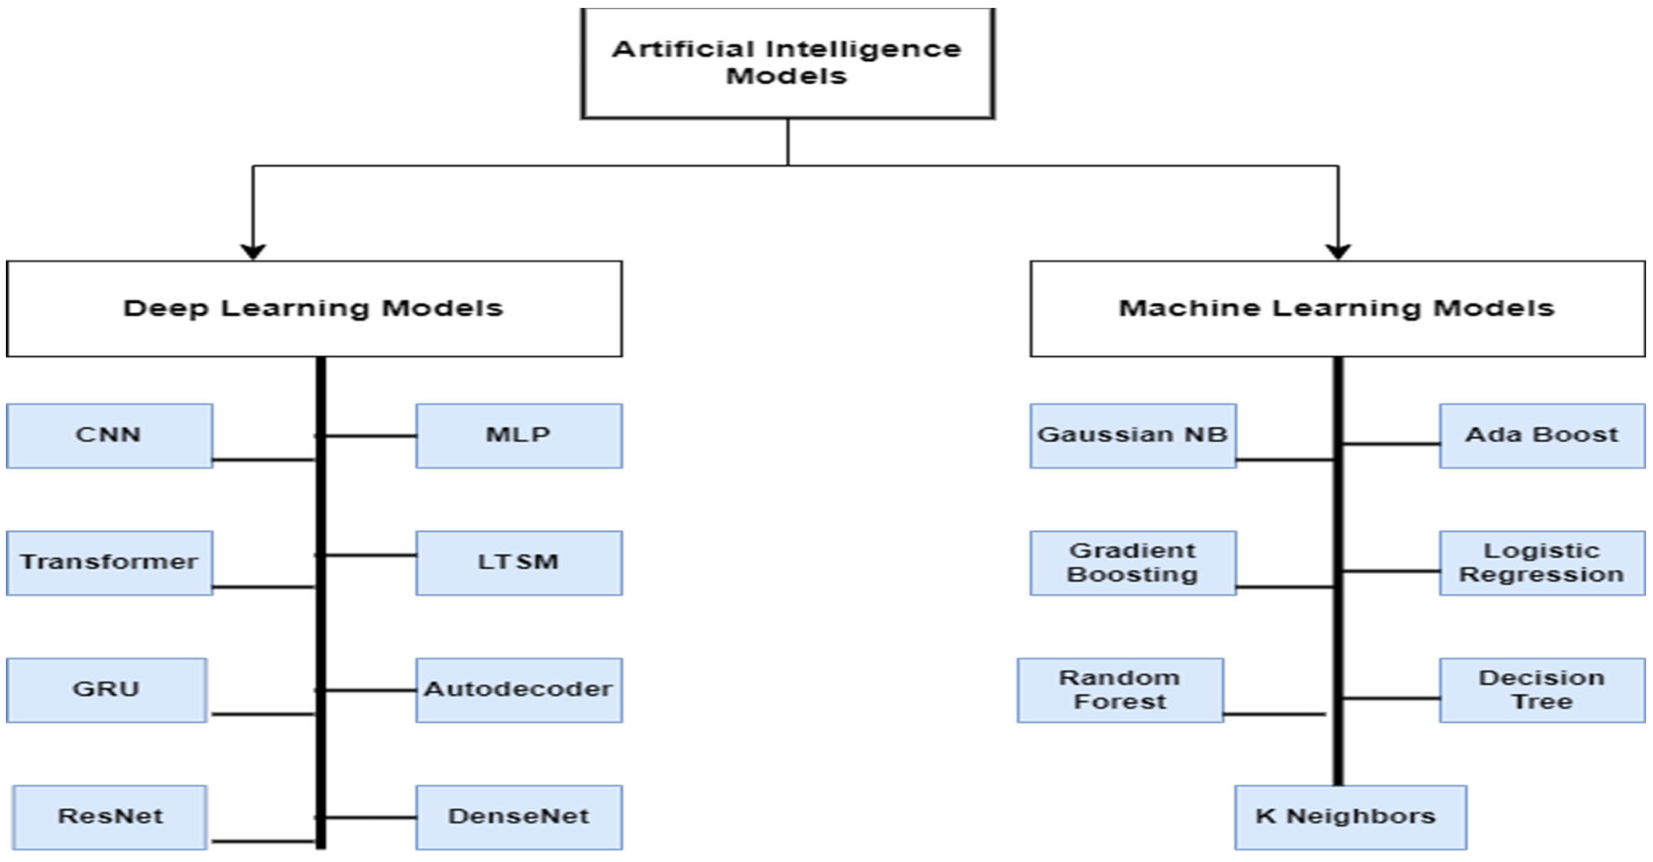
\includegraphics[width=0.66\linewidth,keepaspectratio]{figs/p2_models.png}
   \caption{Deep learning and machine learning models evaluated for loan prediction \cite{p2}}
   \label{fig:p2_models}
\end{figure}

\subsection{Results and Analysis}

\paragraph{} \textbf{Machine learning models.} Table~\ref{tab:p2_ml} shows test results. Random Forest achieves the best overall balance (accuracy 0.90, F1 0.90, AUC 0.91), followed by KNN and Decision Trees. Random Forest and Decision Trees reach 100\% on the training data, a sign of overfitting. The low MCC values of Logistic Regression, Naive Bayes, AdaBoost, and Gradient Boosting (0.06--0.10) despite accuracies of 0.74--0.86 illustrate how accuracy can be misleading on imbalanced data.

{\renewcommand{\arraystretch}{1.2}
\begin{table}[htbp]
\centering
\caption{Test performance of ML models for loan prediction \cite{p2}}\label{tab:p2_ml}
\small
\begin{tabular}{|l|c|c|c|c|c|c|}
\hline
\textbf{Model} & \textbf{Accuracy} & \textbf{Precision} & \textbf{Recall} & \textbf{F1} & \textbf{AUC} & \textbf{MCC} \\ \hline
Gaussian NB & 0.76 & 0.80 & 0.76 & 0.78 & 0.60 & 0.09 \\ \hline
Logistic Regression & 0.86 & 0.80 & 0.86 & 0.82 & 0.62 & 0.07 \\ \hline
AdaBoost & 0.74 & 0.80 & 0.74 & 0.76 & 0.58 & 0.06 \\ \hline
Gradient Boosting & 0.75 & 0.81 & 0.75 & 0.77 & 0.63 & 0.10 \\ \hline
K-Nearest Neighbours & 0.88 & 0.89 & 0.88 & 0.89 & 0.87 & 0.48 \\ \hline
Decision Trees & 0.87 & 0.89 & 0.88 & 0.88 & 0.74 & 0.47 \\ \hline
\textbf{Random Forest} & \textbf{0.90} & \textbf{0.89} & \textbf{0.90} & \textbf{0.90} & \textbf{0.91} & \textbf{0.48} \\ \hline
\end{tabular}
\end{table}}

\paragraph{} \textbf{Deep learning models under different balancing strategies.} Table~\ref{tab:p2_dl} summarises test accuracy and F1-score of the main DL models in five configurations: no balancing, SMOTE-Tomek, SMOTE, ensemble methods only, and ensemble methods with SMOTE. Without balancing, recurrent models (LSTM, GRU, BiLSTM) collapse to predicting the majority class (F1 0.47, AUC 0.51, MCC 0). DenseNet and ResNet are the most accurate models in every configuration, and the combination of ensemble methods with SMOTE gives the best overall result: DenseNet reaches 92\% accuracy, precision, recall, and F1, an AUC of 0.99, and an MCC of 0.64 on the test set. Figure~\ref{fig:p2_chart} visualises the F1-scores.

{\renewcommand{\arraystretch}{1.2}
\begin{table}[htbp]
\centering
\caption{Test accuracy / F1-score (\%) of DL models under different balancing strategies (compiled from \cite{p2})}\label{tab:p2_dl}
\small
\begin{tabular}{|l|c|c|c|c|c|}
\hline
\textbf{Model} & \shortstack{\textbf{No}\\\textbf{balancing}} & \shortstack{\textbf{SMOTE-}\\\textbf{Tomek}} & \textbf{SMOTE} & \textbf{Ensemble} & \shortstack{\textbf{Ensemble}\\\textbf{+ SMOTE}} \\ \hline
DenseNet & 91 / 76 & 91 / 79 & 92 / 82 & 91 / 91 & \textbf{92 / 92} \\ \hline
ResNet & 90 / 73 & 91 / 79 & 91 / 81 & 91 / 90 & 91 / 91 \\ \hline
MLP & 89 / 72 & 89 / 77 & 89 / 77 & 90 / 89 & 90 / 90 \\ \hline
CNN & 89 / 70 & 89 / 77 & 89 / 77 & 89 / 87 & 90 / 90 \\ \hline
LSTM & 88 / 47 & 87 / 47 & 85 / 54 & 88 / 82 & 88 / 83 \\ \hline
\end{tabular}
\end{table}}

\begin{figure}[htbp]
\centering
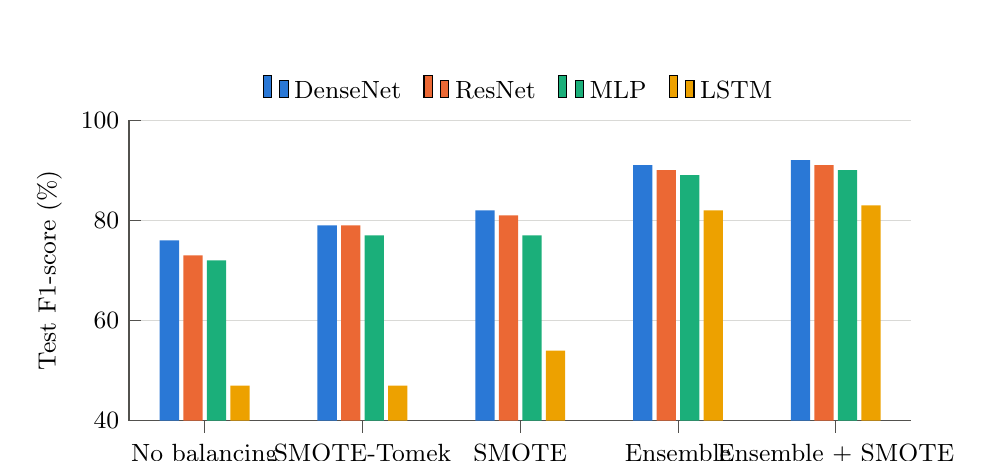
\begin{tikzpicture}
\begin{axis}[
  ybar=1.5pt, bar width=7pt, width=0.95\textwidth, height=5.4cm,
  symbolic x coords={No balancing,SMOTE-Tomek,SMOTE,Ensemble,Ensemble + SMOTE},
  xtick=data, enlarge x limits=0.12, ymin=40, ymax=100,
  ylabel={Test F1-score (\%)}, ylabel style={font=\small},
  ymajorgrids, grid style={gridgray}, axis line style={inkgray}, tick style={inkgray},
  axis x line*=bottom, axis y line*=left, tick label style={font=\small},
  legend style={at={(0.5,1.02)}, anchor=south, legend columns=-1, draw=none, font=\small, /tikz/every even column/.append style={column sep=6pt}},
]
\addplot[fill=seriesA, draw=none] coordinates {(No balancing,76) (SMOTE-Tomek,79) (SMOTE,82) (Ensemble,91) (Ensemble + SMOTE,92)};
\addplot[fill=seriesB, draw=none] coordinates {(No balancing,73) (SMOTE-Tomek,79) (SMOTE,81) (Ensemble,90) (Ensemble + SMOTE,91)};
\addplot[fill=seriesC, draw=none] coordinates {(No balancing,72) (SMOTE-Tomek,77) (SMOTE,77) (Ensemble,89) (Ensemble + SMOTE,90)};
\addplot[fill=seriesD, draw=none] coordinates {(No balancing,47) (SMOTE-Tomek,47) (SMOTE,54) (Ensemble,82) (Ensemble + SMOTE,83)};
\legend{DenseNet, ResNet, MLP, LSTM}
\end{axis}
\end{tikzpicture}
\caption{Test F1-score of selected deep models under each data-balancing configuration, plotted from \cite{p2} (y-axis starts at 40\%)}
\label{fig:p2_chart}
\end{figure}

\subsection{Discussion}

\paragraph{} The paper provides a broad empirical comparison on a large dataset and clearly shows that data balancing and ensembling matter as much as the choice of architecture: the same LSTM moves from a degenerate majority-class predictor to an F1 of 83\% when ensemble methods and SMOTE are added. Densely and residually connected networks were consistently strongest, which the authors attribute to efficient feature reuse and stable gradient flow. Some limitations remain: DenseNet requires more computation and longer training; the results are from a single public dataset; and although the authors emphasise interpretability, SHAP and LIME are discussed as motivation rather than applied to the reported models. The very high training scores of tree models also point to overfitting that should be controlled in deployment.

%---------------------------------------------------------------
\section{Effective Credit Risk Prediction Using Ensemble Classifiers With Model Explanation}

This paper by Aruleba and Sun \cite{p3} combines ensemble classifiers with the hybrid SMOTE-ENN resampling technique to address class imbalance, and uses SHAP to explain the predictions of the best-performing models on two public credit datasets.

\subsection{Problem Statement and Motivation}

\paragraph{} Single classifiers often fail to capture the complexity of credit data, imbalanced datasets bias models toward the majority class, and the black-box nature of ML makes it hard for lenders to justify decisions. The authors argue that combining efficient resampling, ensemble learning, and XAI can address all three problems. Their contributions are to investigate ensemble classifiers for credit risk, demonstrate the benefit of SMOTE-ENN, provide model interpretation with SHAP, and discuss implications for financial institutions.

\subsection{Datasets}

\paragraph{} Two UCI benchmark datasets are used. The \textbf{German Credit} dataset contains 1{,}000 applicants described by attributes such as checking account status, credit amount, duration, age, purpose, savings, housing, job, and sex; about 70\% are labelled ``good'', making it imbalanced. The \textbf{Australian Credit Approval} dataset contains 690 credit card applications with 15 anonymised attributes (A1--A15), with roughly 55\% approved and 45\% denied.

\subsection{Classifiers and Resampling}

\paragraph{} Four ensemble classifiers---\textbf{Random Forest}, \textbf{AdaBoost}, \textbf{XGBoost}, and \textbf{LightGBM}---are compared with three single classifiers: \textbf{CART}, \textbf{Logistic Regression}, and a \textbf{Multi-Layer Perceptron}. Their formulations are those given in Chapter 2. Class imbalance is handled with \textbf{SMOTE-ENN}, summarised in Algorithm~\ref{alg:smoteenn}: SMOTE first creates synthetic minority samples by interpolation (Equation~\ref{eq:smote}), and ENN then removes samples of either class that disagree with the majority of their $k$ nearest neighbours. This both balances the classes and cleans noisy, overlapping boundary regions, so that the resulting decision boundary generalises better.

\begin{algorithm}[htbp]
\caption{SMOTE-ENN resampling (adapted from \cite{p3})}\label{alg:smoteenn}
\begin{algorithmic}[1]
\Require dataset $D$ with minority class $M$ and majority class $N$, over-sampling rate $S$, number of neighbours $k$
\Ensure balanced dataset $D'$
\State Apply SMOTE to $D$ with rate $S$ and $k$ neighbours to generate synthetic samples of $M$
\State $D_{\mathrm{aug}}\gets D\;\cup$ synthetic samples
\State Apply ENN to $D_{\mathrm{aug}}$: remove every sample whose label disagrees with the majority of its $k$ nearest neighbours
\State \Return $D'\gets$ resulting dataset
\end{algorithmic}
\end{algorithm}

\subsection{Proposed Framework}

\paragraph{} The framework has four steps: (1) normalise and encode features and apply SMOTE-ENN to the \emph{training} data only; (2) train Random Forest, AdaBoost, XGBoost, and LightGBM on the balanced data; (3) validate each model with k-fold cross-validation and evaluate accuracy, recall, specificity, and F-measure; and (4) compute SHAP values for the best-performing model to assess feature impact. Specificity is emphasised because it measures how well the model identifies the negative class, which is poorly detected on imbalanced data.

\subsection{Results and Analysis}

\paragraph{} \textbf{German dataset.} Before resampling, every classifier struggled to identify the minority class, with specificity no higher than 0.474; XGBoost had the best accuracy (0.765) and F-measure (0.841) but a specificity of only 0.440 (Table~\ref{tab:p3_german}). After SMOTE-ENN, performance improved substantially. XGBoost reached an accuracy of 0.897, recall of 0.930, specificity of 0.846, and F-measure of 0.907, and Random Forest's specificity rose from 0.430 to 0.825. Figure~\ref{fig:p3_chart} highlights the gain in specificity for every classifier.

{\renewcommand{\arraystretch}{1.2}
\begin{table}[htbp]
\centering
\caption{Classifier performance on the German dataset before and after SMOTE-ENN resampling \cite{p3}}\label{tab:p3_german}
\small
\begin{tabular}{|l|c|c|c|c|c|c|c|c|}
\hline
\multirow{2}{*}{\textbf{Classifier}} & \multicolumn{4}{c|}{\textbf{Before resampling}} & \multicolumn{4}{c|}{\textbf{After SMOTE-ENN}} \\ \cline{2-9}
 & Acc. & Rec. & Spec. & F1 & Acc. & Rec. & Spec. & F1 \\ \hline
AdaBoost & 0.750 & 0.781 & 0.400 & 0.834 & 0.820 & 0.857 & 0.730 & 0.860 \\ \hline
LightGBM & 0.732 & 0.767 & 0.390 & 0.810 & 0.790 & 0.829 & 0.698 & 0.858 \\ \hline
Random Forest & 0.750 & 0.890 & 0.430 & 0.833 & 0.861 & 0.911 & 0.825 & 0.874 \\ \hline
\textbf{XGBoost} & 0.765 & 0.789 & 0.440 & 0.841 & \textbf{0.897} & \textbf{0.930} & \textbf{0.846} & \textbf{0.907} \\ \hline
CART & 0.650 & 0.724 & 0.474 & 0.750 & 0.686 & 0.748 & 0.599 & 0.791 \\ \hline
Logistic Regression & 0.710 & 0.743 & 0.252 & 0.786 & 0.814 & 0.798 & 0.630 & 0.805 \\ \hline
MLP & 0.705 & 0.775 & 0.280 & 0.727 & 0.820 & 0.829 & 0.801 & 0.820 \\ \hline
\end{tabular}
\end{table}}

\begin{figure}[htbp]
\centering
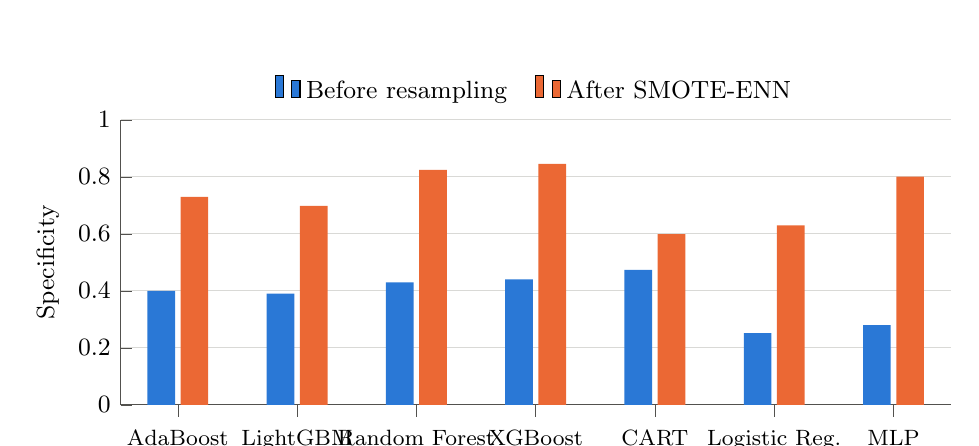
\begin{tikzpicture}
\begin{axis}[
  ybar=2pt, bar width=10pt, width=\textwidth, height=5.2cm,
  symbolic x coords={AdaBoost,LightGBM,Random Forest,XGBoost,CART,Logistic Reg.,MLP},
  xtick=data, enlarge x limits=0.08, ymin=0, ymax=1,
  ylabel={Specificity}, ylabel style={font=\small},
  ymajorgrids, grid style={gridgray}, axis line style={inkgray}, tick style={inkgray},
  axis x line*=bottom, axis y line*=left, tick label style={font=\small}, x tick label style={font=\footnotesize},
  legend style={at={(0.5,1.02)}, anchor=south, legend columns=-1, draw=none, font=\small, /tikz/every even column/.append style={column sep=8pt}},
]
\addplot[fill=seriesA, draw=none] coordinates {(AdaBoost,0.400) (LightGBM,0.390) (Random Forest,0.430) (XGBoost,0.440) (CART,0.474) (Logistic Reg.,0.252) (MLP,0.280)};
\addplot[fill=seriesB, draw=none] coordinates {(AdaBoost,0.730) (LightGBM,0.698) (Random Forest,0.825) (XGBoost,0.846) (CART,0.599) (Logistic Reg.,0.630) (MLP,0.801)};
\legend{Before resampling, After SMOTE-ENN}
\end{axis}
\end{tikzpicture}
\caption{Specificity on the German Credit dataset before and after SMOTE-ENN, plotted from \cite{p3}}
\label{fig:p3_chart}
\end{figure}

\paragraph{} \textbf{Australian dataset.} This dataset is nearly balanced, so all models performed reasonably even before resampling, with XGBoost best (accuracy 0.895, recall 0.870, F-measure 0.886). After SMOTE-ENN, Random Forest improved the most and became the best model, with accuracy 0.916, recall 0.907, specificity 0.922, and F-measure 0.910; XGBoost followed closely (0.910, 0.898, 0.914, 0.903), and CART remained the weakest (accuracy 0.829).

\paragraph{} \textbf{Model explanation with SHAP.} Figure~\ref{fig:p3_shap} shows SHAP summary plots for the best models. For XGBoost on German Credit, \emph{checking account} is the most influential feature, with higher values pushing predictions toward good credit; \emph{credit amount}, \emph{duration}, and \emph{age} have mixed positive and negative effects, suggesting interactions with other features; and \emph{purpose}, \emph{savings}, \emph{housing}, \emph{job}, and \emph{sex} have smaller impact. For Random Forest on the Australian data, attribute A9 dominates, followed by A15, A11, and A8.

\begin{figure}[htbp]
\centering
\begin{subfigure}[b]{0.49\textwidth}
  \centering
  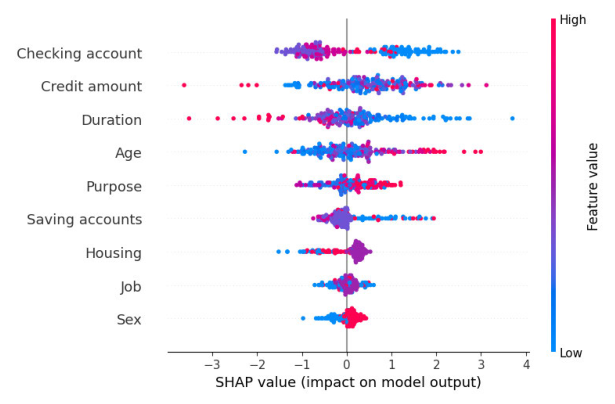
\includegraphics[width=\linewidth,keepaspectratio]{figs/p3_shap_german.png}
  \caption{XGBoost, German Credit}
\end{subfigure}\hfill
\begin{subfigure}[b]{0.43\textwidth}
  \centering
  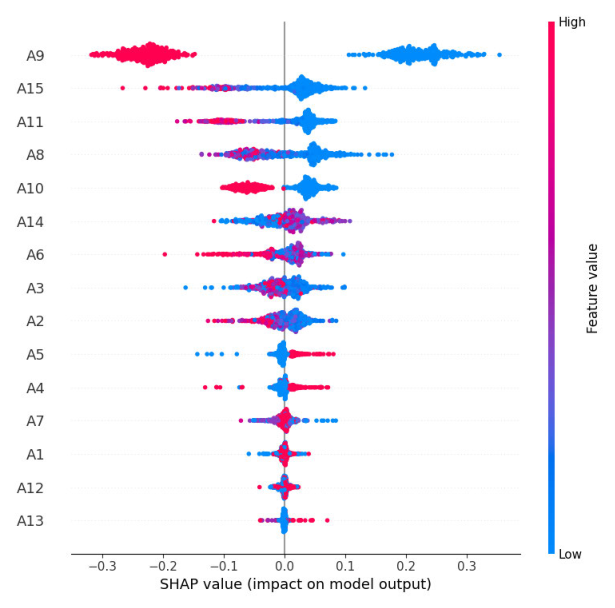
\includegraphics[width=\linewidth,keepaspectratio]{figs/p3_shap_australian.png}
  \caption{Random Forest, Australian Credit}
\end{subfigure}
\caption{SHAP summary plots of the best-performing models; red indicates high and blue low feature values \cite{p3}}
\label{fig:p3_shap}
\end{figure}

\paragraph{} \textbf{Comparison with prior work.} On the Australian dataset the proposed Random Forest with SMOTE-ENN (accuracy 0.916, specificity 0.922) compares favourably with earlier methods such as a CART-based majority-voting ensemble (accuracy 0.913, recall 0.953, specificity 0.871), and on the German dataset it outperforms most earlier approaches, including gradient-boosted trees with SMOTE (accuracy 0.824). The authors stress that, unlike nearly all compared studies, their approach also provides interpretability.

\subsection{Discussion}

\paragraph{} The paper shows clearly that resampling matters most on strongly imbalanced data: specificity on German Credit roughly doubled for every classifier after SMOTE-ENN. It also demonstrates a practical, reproducible pipeline that pairs strong ensembles with SHAP explanations. Its limitations are the small size of the benchmark datasets (1{,}000 and 690 instances), the anonymised features of the Australian data, which limit the practical meaning of its explanations, and the absence of any fairness analysis even though the German data includes sensitive attributes such as age and sex. The authors suggest testing on more diverse and larger datasets.

%---------------------------------------------------------------
\section{Explainable and Fair AI: Balancing Performance in Financial and Real Estate Machine Learning Models}

This paper by Acharya, Divya, and Kuppan \cite{p4} presents a framework that integrates fairness constraints and explainability into gradient boosting models (LightGBM and XGBoost) for loan approval and house price prediction, and studies the trade-off between accuracy, fairness, and interpretability.

\subsection{Problem Statement and Motivation}

\paragraph{} Fairness and explainability have been studied extensively in healthcare and criminal justice, but much less in finance and real estate, even though decisions in these domains shape access to credit and housing. Biased models can deny loans or misprice homes for particular groups, and regulators increasingly demand that automated decisions be accurate, understandable, and fair. The authors therefore apply fairness techniques---\textbf{Calibrated Equalized Odds} and \textbf{Intersectional Fairness}---together with SHAP, LIME, PDP, and ALE explanations, to two high-stakes prediction tasks.

\subsection{Methodology}

\paragraph{} \textbf{Data and preprocessing.} A loan approval dataset (applicant and co-applicant income, loan amount and term, credit history, property area, and demographic attributes such as gender, marital status, education, and dependents) and a house price dataset (overall quality, living area, neighbourhood, basement and garage attributes) are used. Missing numerical values are imputed with the mean and categorical values with the mode, features such as the loan-to-income ratio are engineered, and numerical features are normalised.

\paragraph{} \textbf{Models.} LightGBM and XGBoost are trained on 80\% of the data and tested on 20\%, with grid search over learning rate, number of trees, and maximum depth.

\paragraph{} \textbf{Fairness constraints.} Fairness is evaluated for groups defined by gender and income level (loans) and location and property size (housing). \textbf{Calibrated Equalized Odds} post-processes model outputs to equalise false-positive and false-negative rates across groups while preserving calibration, and \textbf{Intersectional Fairness} assesses combinations of protected attributes. Fairness is measured with \textbf{Disparate Impact} and \textbf{Equal Opportunity Difference}.

\paragraph{} \textbf{Explainability.} SHAP summary plots provide global feature rankings and SHAP force plots explain individual predictions; LIME provides local explanations; PDPs and ALE plots visualise feature effects; and a \emph{fairness-aware SHAP} analysis examines how demographic features influence predictions and highlights when predictions deviate from fairness expectations.

\subsection{Results and Analysis}

\paragraph{} \textbf{Loan approval performance.} LightGBM outperformed XGBoost on every metric (Table~\ref{tab:p4_perf}), with accuracy 0.80, precision 0.81, recall 0.9375, and F1-score 0.857. The authors report that LightGBM also balanced accuracy and fairness better than XGBoost, and that applying Calibrated Equalized Odds reduced accuracy slightly but mitigated gender bias.

{\renewcommand{\arraystretch}{1.2}
\begin{table}[htbp]
\centering
\caption{Performance of loan approval models \cite{p4}}\label{tab:p4_perf}
\small
\begin{tabular}{|l|c|c|c|c|}
\hline
\textbf{Model} & \textbf{Accuracy} & \textbf{Precision} & \textbf{Recall} & \textbf{F1-score} \\ \hline
\textbf{LightGBM} & \textbf{0.80} & \textbf{0.81} & \textbf{0.9375} & \textbf{0.857} \\ \hline
XGBoost & 0.79 & 0.80 & 0.937 & 0.842 \\ \hline
\end{tabular}
\end{table}}

\paragraph{} \textbf{Global explanations.} The SHAP summary plot for LightGBM on loan approval (Figure~\ref{fig:p4_shap}) shows \emph{Credit History} as by far the most influential feature, followed by \emph{Loan Amount} and \emph{Applicant Income}; demographic features such as gender and education have small SHAP values. XGBoost produces a similar ranking. For house prices, \emph{Overall Quality} and \emph{GrLivArea} (above-ground living area) dominate for both models (Figure~\ref{fig:p4_house}).

\begin{figure}[htbp]
   \centering
   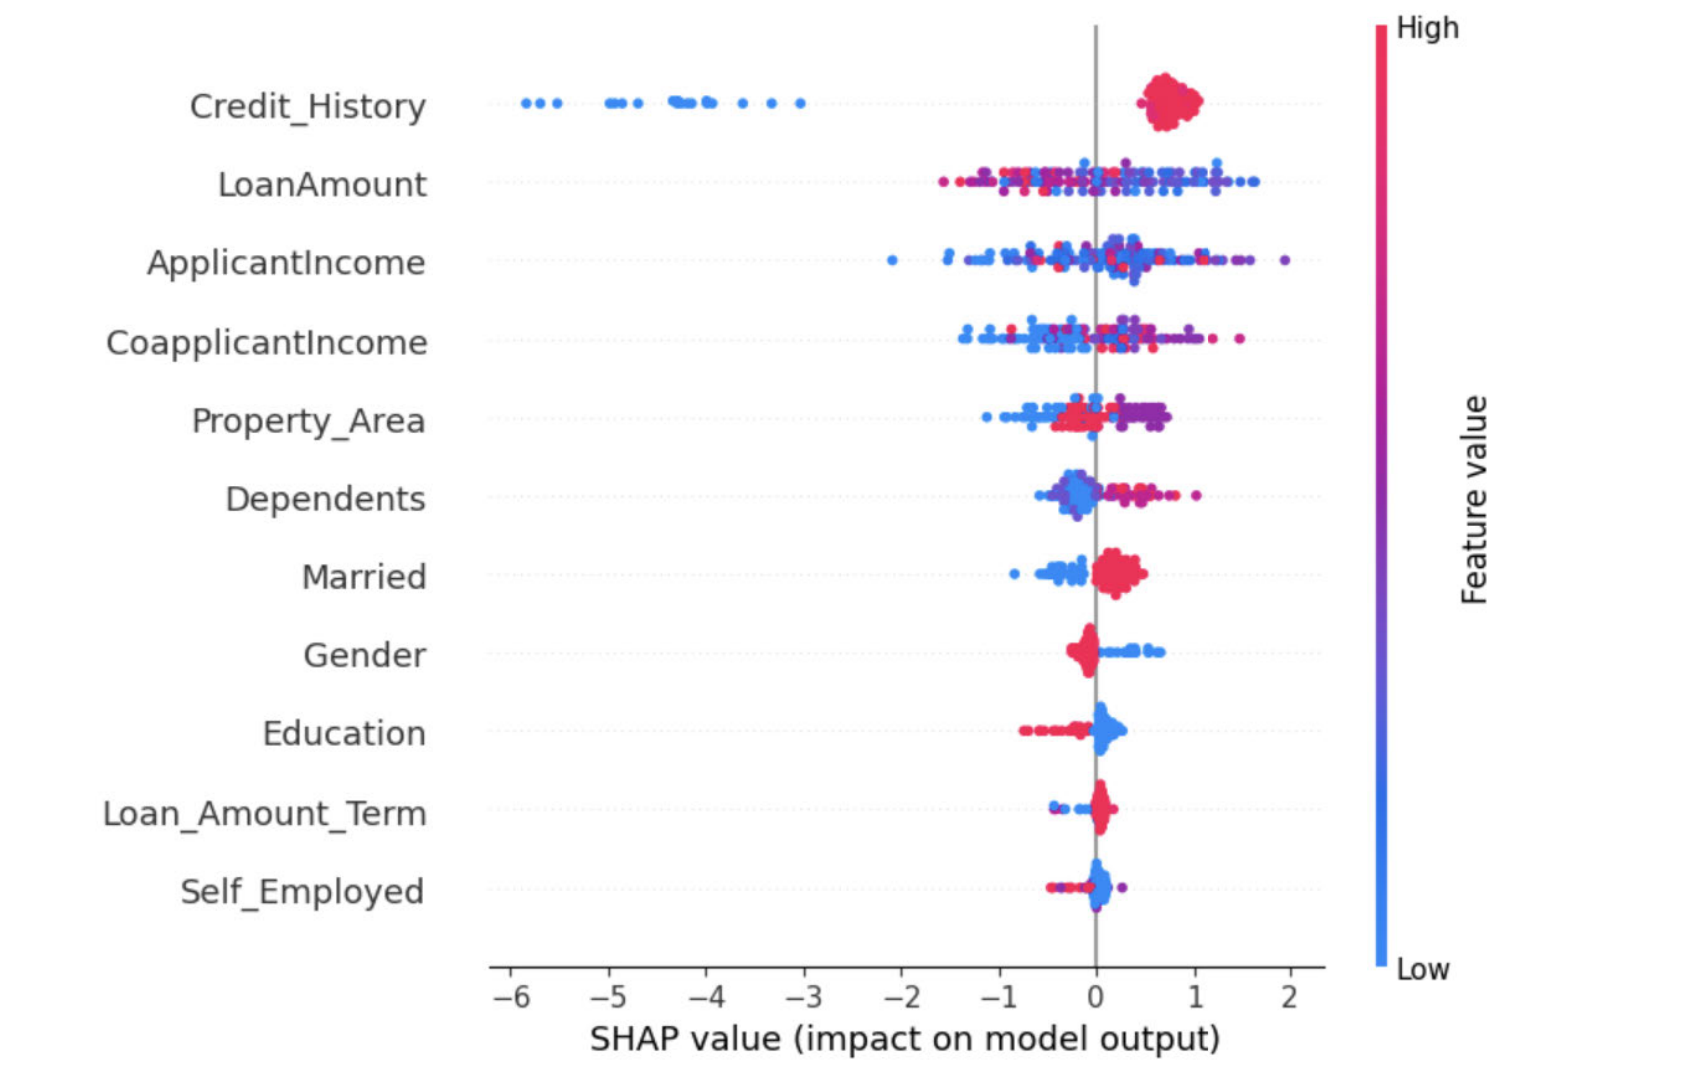
\includegraphics[width=0.66\linewidth,keepaspectratio]{figs/p4_shap_lgbm_loan.png}
   \caption{SHAP summary plot for LightGBM on the loan approval dataset \cite{p4}}
   \label{fig:p4_shap}
\end{figure}

\paragraph{} \textbf{Local explanations.} SHAP force plots show how credit history and loan amount pushed an individual application toward approval, and LIME explanations (Figure~\ref{fig:p4_lime}) show the contribution of specific feature values---such as a co-applicant income of zero or a loan amount above a threshold---to a single decision.

\begin{figure}[htbp]
   \centering
   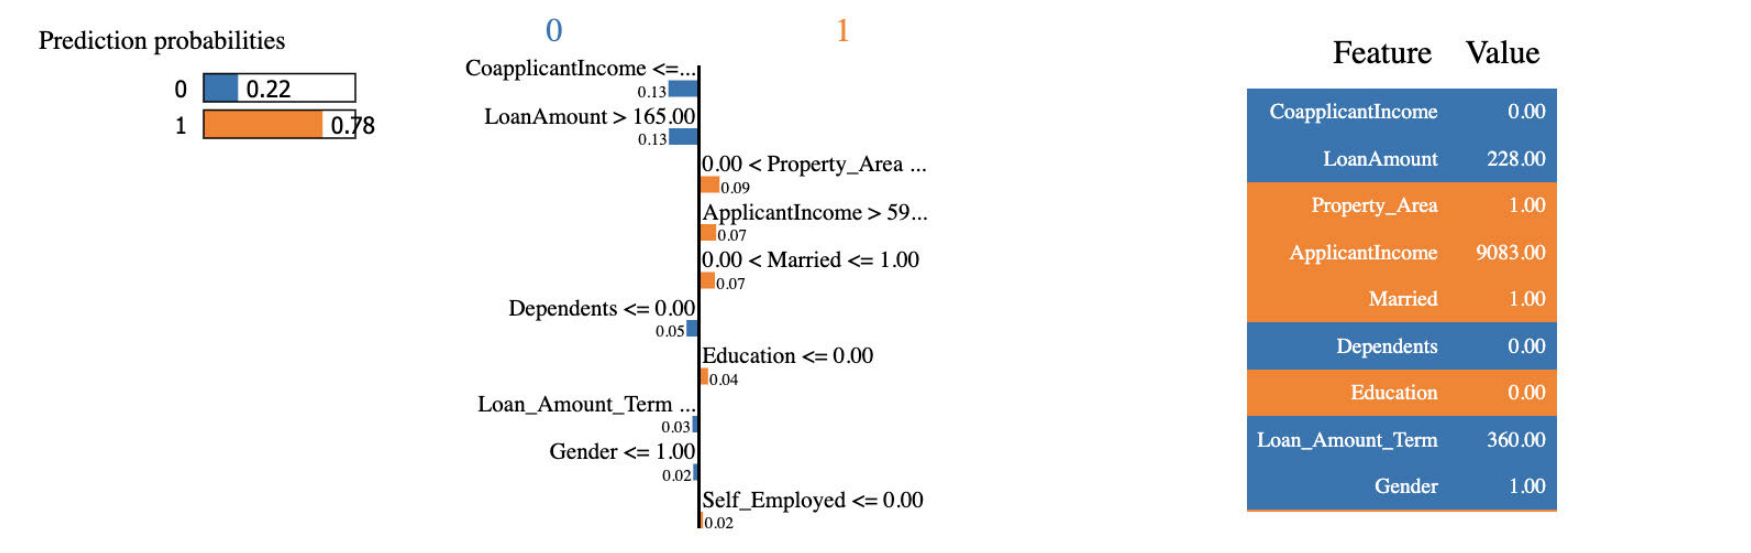
\includegraphics[width=0.82\linewidth,keepaspectratio]{figs/p4_lime_loan.png}
   \caption{LIME explanation of a single loan approval prediction by LightGBM \cite{p4}}
   \label{fig:p4_lime}
\end{figure}

\begin{figure}[htbp]
   \centering
   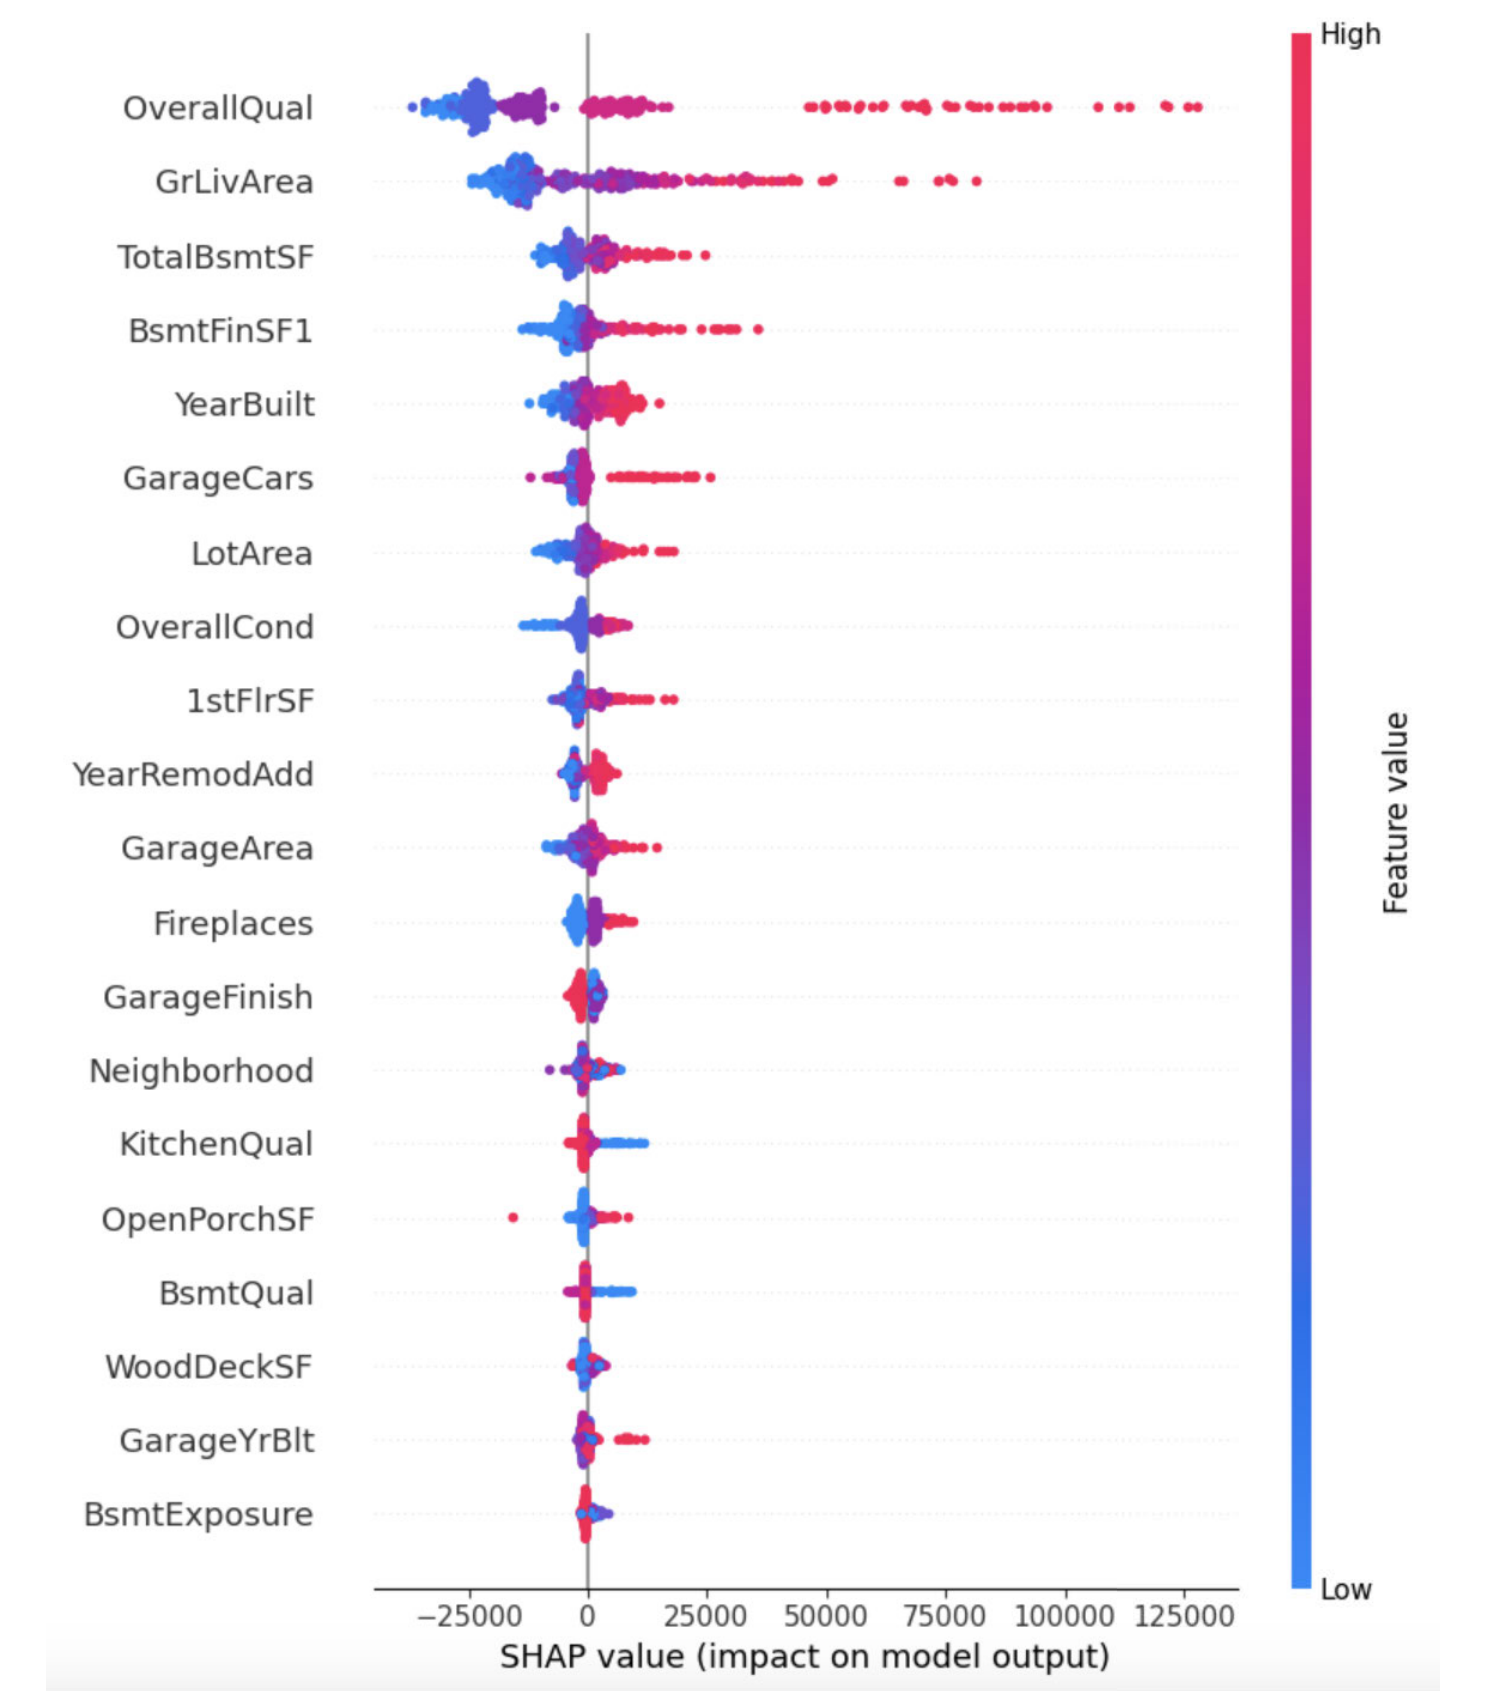
\includegraphics[width=0.46\linewidth,keepaspectratio]{figs/p4_shap_house.png}
   \caption{SHAP summary plot for LightGBM on the house price dataset \cite{p4}}
   \label{fig:p4_house}
\end{figure}

\paragraph{} \textbf{SHAP versus LIME.} Table~\ref{tab:p4_shaplime} summarises the authors' comparison. Both methods identify the same most important features, but SHAP provides consistent global and local attributions, whereas LIME gives intuitive, instance-level explanations; the two are therefore complementary.

{\renewcommand{\arraystretch}{1.2}
\begin{table}[htbp]
\centering
\caption{Comparison of SHAP and LIME as observed in \cite{p4}}\label{tab:p4_shaplime}
\small
\begin{tabularx}{\textwidth}{|p{3.2cm}|X|X|}
\hline
\textbf{Aspect} & \textbf{SHAP} & \textbf{LIME} \\ \hline
Scope & Global ranking and local attributions & Primarily local, per-instance \\ \hline
Theoretical basis & Shapley values from cooperative game theory; additive & Local surrogate model fitted on perturbed samples \\ \hline
Detail & Granular feature contributions, including interactions & Which feature values pushed one prediction up or down \\ \hline
Typical use & Model audit, feature importance, regulatory reporting & Explaining a single decision to a customer or officer \\ \hline
\end{tabularx}
\end{table}}

\subsection{Contributions and Discussion}

\paragraph{} The paper's main contributions are the application of Calibrated Equalized Odds and intersectional fairness in finance and real estate, the dual use of SHAP across two domains, and a benchmark of fairness-aware LightGBM and XGBoost that shows fairness and accuracy can coexist with only a small loss in performance. It also relates the framework to AI governance and the GDPR's right to explanation. However, the fairness results are reported qualitatively rather than as numeric DI and EOD values, fairness is analysed only with respect to gender, and the datasets are relatively small, structured tables. The authors propose adversarial fairness, genuine intersectional analysis, fairness-aware explanation tools, and extension to multimodal data as future work.

\section{Summary of the Reviewed Papers}

\paragraph{} Table~\ref{tab:summary} summarises the four papers reviewed in this chapter---their venue, task, main technique, data, and headline result. The next chapter compares them in detail.

{\renewcommand{\arraystretch}{1.2}
\begin{table}[htbp]
\centering
\caption{Summary of the reviewed papers}\label{tab:summary}
\small
\begin{tabularx}{\textwidth}{|p{0.85cm}|p{2.1cm}|X|p{2.7cm}|X|}
\hline
\textbf{Ref.} & \textbf{Venue} & \textbf{Main technique} & \textbf{Data} & \textbf{Headline result} \\ \hline
\cite{p1} & IEEE Access, vol. 13, 2025 & Hybrid LSTM network, hybrid loss, SMOTE, SHAP, fairness regulariser & German Credit, GMSC, CreditRisk & AUC 85.30\% / 90.56\%; EOD 0.036 \\ \hline
\cite{p2} & IEEE Access, vol. 12, 2024 & 7 ML + 9 DL models; SMOTE, SMOTE-Tomek, ensembles & 252{,}000 bank records & DenseNet 92\% accuracy and F1 \\ \hline
\cite{p3} & IEEE Access, vol. 12, 2024 & RF, AdaBoost, XGBoost, LightGBM; SMOTE-ENN; SHAP & German, Australian Credit & XGBoost 0.897 / RF 0.916 accuracy \\ \hline
\cite{p4} & IEEE Access, vol. 12, 2024 & LightGBM, XGBoost; Calibrated Equalized Odds; SHAP, LIME & Loan approval, house prices & LightGBM F1 0.857 with fairness \\ \hline
\end{tabularx}
\end{table}}


% ================= CHAPTER 4: DISCUSSION & COMPARISON =================
\chapter{Discussion \& Comparison}

\paragraph{} This chapter compares the four reviewed papers. Although all address credit risk or loan approval, they emphasise different parts of the pipeline---deep architectures, large-scale model comparison, resampling with ensembles, and fairness with explainability---and evaluate on different datasets. The comparison below highlights their complementary strengths and the trade-offs among accuracy, robustness to imbalance, interpretability, and fairness.

\section{Analytical Focus}

\paragraph{} Paper \cite{p1} focuses on \textbf{architecture design}, building a hybrid LSTM-based network that integrates structured and behavioural data and embeds interpretability and fairness into its loss. Paper \cite{p2} focuses on \textbf{empirical model selection}, comparing sixteen ML and DL models under five data-balancing configurations on a large bank dataset. Paper \cite{p3} focuses on \textbf{imbalance handling with explanation}, showing how SMOTE-ENN transforms the performance of ensemble classifiers and how SHAP reveals their decision logic. Paper \cite{p4} focuses on \textbf{responsible AI}, adding fairness constraints and multiple explanation methods to gradient boosting models in finance and real estate.

\section{Comparison of Methodologies}

\paragraph{} Table~\ref{tab:compare} summarises the methodology, advantages, and limitations of each paper.

{\renewcommand{\arraystretch}{1.35}
\setlength{\tabcolsep}{6pt}
\small
\begin{longtable}{|p{3.1cm}|p{3.65cm}|p{3.65cm}|p{3.65cm}|}
\caption{Comparison of the reviewed approaches}\label{tab:compare}\\
\hline
\textbf{Paper} & \textbf{Methodology} & \textbf{Advantages} & \textbf{Limitations} \\ \hline
\endfirsthead
\hline
\textbf{Paper} & \textbf{Methodology} & \textbf{Advantages} & \textbf{Limitations} \\ \hline
\endhead
\hline
\endfoot
\hline
\endlastfoot
Credit scoring prediction using deep learning \cite{p1} &
Feature transformation + LSTM/dense hybrid network; L1 hybrid loss; adaptive regularisation; SMOTE and weighted loss; SHAP and tree distillation; fairness regulariser. &
Integrates behavioural sequences; best AUC on German (85.30\%) and GMSC (90.56\%); EOD reduced from 0.124 to 0.036. &
Much of the evaluation uses text datasets; needs rich behavioural data; deep model still less transparent than a scorecard. \\ \hline
ML and DL for loan prediction \cite{p2} &
7 ML and 9 DL classifiers; SMOTE, SMOTE-Tomek, and ensemble methods; Adam optimisation; 252{,}000-record bank dataset. &
Broad benchmark on large data; DenseNet with ensemble + SMOTE reaches 92\% accuracy and F1, AUC 0.99. &
Single dataset; interpretability not applied to results; tree models overfit training data; DenseNet is computationally heavy. \\ \hline
Ensemble classifiers with model explanation \cite{p3} &
RF, AdaBoost, XGBoost, LightGBM vs.\ CART, LR, MLP; SMOTE-ENN resampling; k-fold validation; SHAP summary plots. &
Specificity roughly doubled on German data; XGBoost 0.897 accuracy (German); RF 0.916 (Australian); interpretable results. &
Small datasets; anonymised Australian features; no fairness analysis despite sensitive attributes. \\ \hline
Explainable and fair AI \cite{p4} &
LightGBM and XGBoost; Calibrated Equalized Odds and intersectional fairness; SHAP, LIME, PDP, ALE; DI and EOD metrics. &
Explicit fairness constraints; complementary global and local explanations; cross-domain (loans and housing). &
Fairness results mostly qualitative; only gender analysed; small structured datasets. \\
\end{longtable}}

\section{Techniques Used}

\paragraph{} Table~\ref{tab:techniques} shows which techniques each paper uses. No paper covers every stage of the pipeline: \cite{p1} is the most complete but evaluates mostly on non-credit data, while \cite{p2} and \cite{p3} provide strong empirical evidence on credit data but little or no fairness analysis.

{\renewcommand{\arraystretch}{1.2}
\begin{table}[htbp]
\centering
\caption{Techniques used in each reviewed paper ($\checkmark$ = used)}\label{tab:techniques}
\small
\begin{tabular}{|l|c|c|c|c|}
\hline
\textbf{Technique} & \textbf{\cite{p1}} & \textbf{\cite{p2}} & \textbf{\cite{p3}} & \textbf{\cite{p4}} \\ \hline
Classical ML baselines (LR, trees, NB, KNN) & \checkmark & \checkmark & \checkmark & -- \\ \hline
Ensemble learning (RF, boosting) & \checkmark & \checkmark & \checkmark & \checkmark \\ \hline
Deep learning (MLP, CNN, LSTM, ResNet, DenseNet) & \checkmark & \checkmark & \checkmark (MLP) & -- \\ \hline
Oversampling (SMOTE) & \checkmark & \checkmark & \checkmark & -- \\ \hline
Hybrid resampling (SMOTE-Tomek / SMOTE-ENN) & -- & \checkmark & \checkmark & -- \\ \hline
Cost-sensitive / focal loss & \checkmark & -- & -- & -- \\ \hline
SHAP explanations & \checkmark & -- & \checkmark & \checkmark \\ \hline
LIME, PDP, ALE & -- & -- & -- & \checkmark \\ \hline
Interpretable-by-design (sparsity, distillation) & \checkmark & -- & -- & -- \\ \hline
Fairness metrics and constraints & \checkmark & -- & -- & \checkmark \\ \hline
\end{tabular}
\end{table}}

\section{Datasets and Evaluation}

\paragraph{} The papers evaluate on different data, summarised in Table~\ref{tab:datasets}. This makes direct numerical comparison across papers inappropriate: an accuracy of 0.90 on a 252{,}000-record dataset with a strongly imbalanced target is not comparable to 0.90 on the 690-record, nearly balanced Australian dataset. Within each paper, however, the comparisons are controlled and informative.

{\renewcommand{\arraystretch}{1.2}
\begin{table}[htbp]
\centering
\caption{Datasets and metrics used by the reviewed papers}\label{tab:datasets}
\small
\begin{tabularx}{\textwidth}{|p{1.2cm}|X|X|}
\hline
\textbf{Paper} & \textbf{Datasets} & \textbf{Metrics} \\ \hline
\cite{p1} & German Credit (1{,}000); Give Me Some Credit ($>$150{,}000); CreditRisk; THUCNews, SciHTC, UTCD (text) & Accuracy, precision, F1, AUC, EOD \\ \hline
\cite{p2} & Kaggle bank loan dataset (252{,}000 records, 13 features) & Accuracy, precision, recall, F1, AUC-ROC, MCC \\ \hline
\cite{p3} & German Credit (1{,}000); Australian Credit Approval (690) & Accuracy, recall, specificity, F-measure \\ \hline
\cite{p4} & Loan approval dataset; house price dataset & Accuracy, precision, recall, F1, DI, EOD \\ \hline
\end{tabularx}
\end{table}}

\section{Model Performance}

\paragraph{} Within their own settings, the papers report the following best results:
\begin{itemize}
  \item Paper \cite{p1}: AUC of 85.30\% (German) and 90.56\% (GMSC), about 2.2 and 2.3 points above LightGBM, and 92.10\% AUC with EOD 0.036 in the full ablation configuration.
  \item Paper \cite{p2}: DenseNet with ensemble methods and SMOTE achieves 92\% test accuracy, precision, recall, and F1, AUC 0.99, and MCC 0.64; Random Forest is the best ML model with 90\% accuracy.
  \item Paper \cite{p3}: XGBoost with SMOTE-ENN achieves 0.897 accuracy, 0.930 recall, and 0.846 specificity on German Credit; Random Forest achieves 0.916 accuracy and 0.922 specificity on Australian Credit.
  \item Paper \cite{p4}: LightGBM achieves 0.80 accuracy, 0.9375 recall, and 0.857 F1 on loan approval while satisfying fairness constraints.
\end{itemize}
A consistent finding is that \textbf{gradient-boosted ensembles and densely connected deep networks} are the strongest model families, and that \textbf{data balancing} changes results as much as model choice does. On German Credit, where two papers overlap, the hybrid deep model of \cite{p1} and XGBoost with SMOTE-ENN of \cite{p3} both clearly surpass standard logistic regression and random forest baselines.

\section{Handling Class Imbalance}

\paragraph{} All three papers that address imbalance agree that it must be handled explicitly. Paper \cite{p2} shows the most dramatic effect: recurrent networks trained on unbalanced data predict only the majority class (MCC 0), while ensembles with SMOTE raise their F1 to above 80\%. Paper \cite{p3} shows that hybrid resampling with cleaning (SMOTE-ENN) roughly doubles specificity on the imbalanced German data but changes little on the balanced Australian data, confirming that the benefit depends on the degree of imbalance. Paper \cite{p1} combines several mechanisms---SMOTE, class weights, focal loss, and hard example mining---and finds in its ablation that SMOTE improves both accuracy and fairness. A general lesson is that resampling must be restricted to training folds to avoid optimistic bias.

\section{Interpretability}

\paragraph{} The papers illustrate three complementary routes to interpretability. \textbf{Post-hoc attribution} with SHAP (\cite{p1}, \cite{p3}, \cite{p4}) explains any model and provides both global rankings and local explanations; it consistently highlights intuitive drivers such as checking-account status, credit history, loan amount, and income. \textbf{Local surrogates} with LIME (\cite{p4}) give simple, instance-specific explanations suitable for customer communication. \textbf{Interpretability by design} (\cite{p1}) uses an L1 sparsity term and distils the network into a decision tree, so that the model itself relies on fewer features and can be summarised as rules. Paper \cite{p2}, despite motivating interpretability, reports no explanations, which illustrates how easily transparency is neglected in accuracy-focused studies.

\section{Fairness}

\paragraph{} Only two papers measure fairness. Paper \cite{p1} integrates a fairness-aware regulariser and reports a quantitative reduction in Equal Opportunity Difference from 0.124 to 0.036, with nearly equal F1-scores across age groups. Paper \cite{p4} applies Calibrated Equalized Odds post-processing and intersectional analysis, and reports that fairness can be improved with only a small loss in accuracy, though without numeric fairness values. Papers \cite{p2} and \cite{p3} use datasets that contain sensitive attributes such as age, sex, and marital status but do not evaluate fairness at all. Given the legal and ethical stakes of lending, fairness auditing should become a standard part of credit model evaluation.

\section{Accuracy--Interpretability Design Space}

\paragraph{} Figure~\ref{fig:design} places the main model families in a qualitative accuracy--interpretability space. Logistic regression and single trees are highly interpretable but less accurate; boosted ensembles and deep networks are more accurate but opaque. XAI and fairness techniques move complex models toward the upper-right region, where accuracy is high and decisions can still be explained and audited---the target of all four reviewed papers.

\begin{figure}[htbp]
\centering
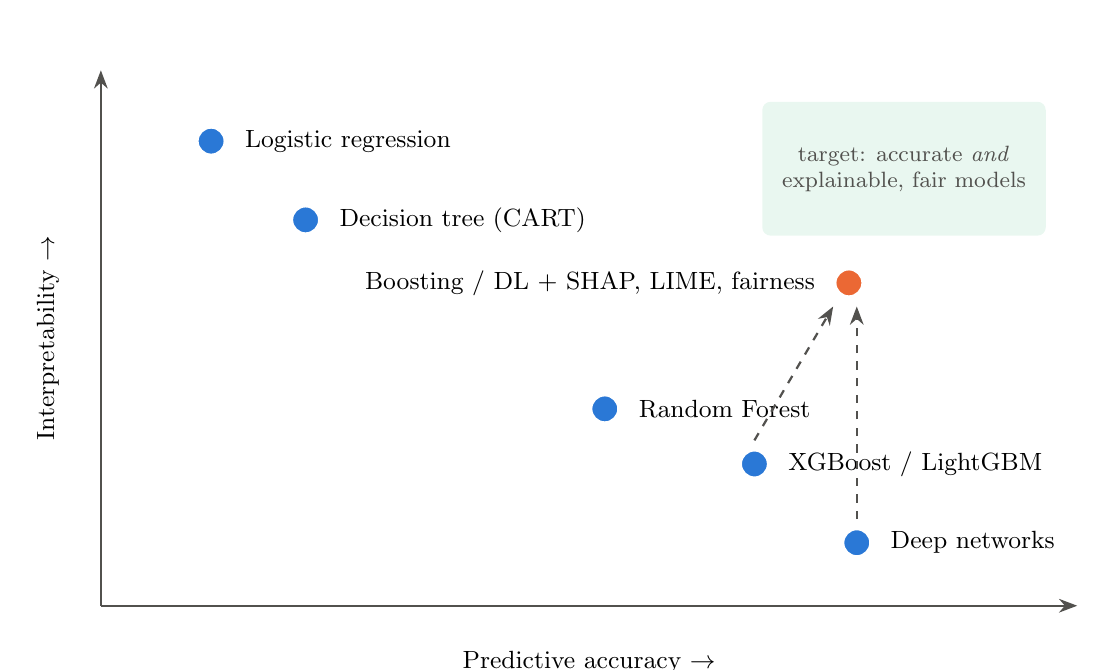
\begin{tikzpicture}[>=Stealth, thick]
\fill[boxgreen!70, rounded corners=3pt] (8.4,4.7) rectangle (12.0,6.4);
\node[font=\footnotesize, align=center, text=inkgray] at (10.2,5.55) {target: accurate \emph{and}\\explainable, fair models};
\draw[->, inkgray] (0,0) -- (12.4,0);
\draw[->, inkgray] (0,0) -- (0,6.8);
\node[font=\small, anchor=north] at (6.2,-0.45) {Predictive accuracy $\rightarrow$};
\node[font=\small, anchor=south, rotate=90] at (-0.4,3.4) {Interpretability $\rightarrow$};
\filldraw[fill=seriesA, draw=white, line width=1pt] (1.4,5.9) circle (5pt); \node[font=\small, anchor=west] at (1.7,5.9) {Logistic regression};
\filldraw[fill=seriesA, draw=white, line width=1pt] (2.6,4.9) circle (5pt); \node[font=\small, anchor=west] at (2.9,4.9) {Decision tree (CART)};
\filldraw[fill=seriesA, draw=white, line width=1pt] (6.4,2.5) circle (5pt); \node[font=\small, anchor=west] at (6.7,2.5) {Random Forest};
\filldraw[fill=seriesA, draw=white, line width=1pt] (8.3,1.8) circle (5pt); \node[font=\small, anchor=west] at (8.6,1.8) {XGBoost / LightGBM};
\filldraw[fill=seriesA, draw=white, line width=1pt] (9.6,0.8) circle (5pt); \node[font=\small, anchor=west] at (9.9,0.8) {Deep networks};
\filldraw[fill=seriesB, draw=white, line width=1pt] (9.5,4.1) circle (5pt); \node[font=\small, anchor=east] at (9.2,4.1) {Boosting / DL + SHAP, LIME, fairness};
\draw[->, dashed, inkgray] (8.3,2.1) -- (9.3,3.8);
\draw[->, dashed, inkgray] (9.6,1.1) -- (9.6,3.8);
\end{tikzpicture}
\caption{Qualitative positioning of model families in an accuracy--interpretability space. Positions are a qualitative synthesis, not measured values.}
\label{fig:design}
\end{figure}

\section{Overall Comparative Insights}

\paragraph{} In synthesis, paper \cite{p1} shows how interpretability and fairness can be built into a deep architecture, paper \cite{p2} shows which architectures and balancing strategies work best at scale, paper \cite{p3} shows how resampling and SHAP combine into a strong and explainable pipeline, and paper \cite{p4} shows how fairness constraints and multiple explanation tools can be added to gradient boosting with little loss of accuracy. A trustworthy credit model should therefore combine a strong learner, explicit imbalance handling, global and local explanations, and quantitative fairness evaluation.

% ================= CHAPTER 5: APPLICATIONS =================
\chapter{Applications}

\paragraph{} Interpretable and fair credit risk models have many practical applications across the financial sector and beyond. This chapter outlines the most important ones and relates them to the reviewed papers.

\section{Retail Loan Approval}

\paragraph{} The most direct application is automated assessment of personal, education, vehicle, and home loan applications. Models such as those in \cite{p2} and \cite{p3} can screen large volumes of applications in seconds, flag high-risk applicants, and route borderline cases to human officers. SHAP and LIME explanations allow officers to see why a model recommends approval or rejection, and to communicate the main reasons to applicants.

\section{Credit Cards and Digital Lending}

\paragraph{} Credit card approval, credit limit setting, and instant digital loans require fast decisions on thin credit files. Deep models that exploit transaction and behavioural sequences, as in \cite{p1}, can assess applicants with limited traditional credit history, while resampling techniques keep the rare default class properly represented.

\section{Financial Inclusion and Microfinance}

\paragraph{} Many people, especially in developing economies, lack formal credit histories. Models that use alternative data---payment of utility bills, mobile transactions, or spending behaviour---can extend credit responsibly to these groups. Fairness auditing, as in \cite{p1} and \cite{p4}, is especially important here to ensure that new models do not reproduce historical exclusion.

\section{Real Estate and Mortgage Lending}

\paragraph{} Paper \cite{p4} applies the same fairness and explainability framework to house price prediction. Transparent valuation models support mortgage underwriting, property taxation, and investment decisions, and fairness constraints help prevent systematic under-valuation of properties in particular neighbourhoods.

\section{Regulatory Compliance and Model Risk Management}

\paragraph{} Banks must validate and document their models for supervisors and auditors. Global SHAP rankings, surrogate decision trees, and fairness metrics such as Disparate Impact and Equal Opportunity Difference provide evidence that a model behaves sensibly and does not discriminate, supporting compliance with data-protection rules such as the GDPR and with fair-lending principles.

\section{Portfolio Monitoring and Early Warning}

\paragraph{} Beyond origination, the same models can monitor existing borrowers and provide early warning of rising default risk, allowing lenders to offer restructuring or support before a loan becomes non-performing. Temporal models such as the LSTM-based architecture of \cite{p1} are well suited to such monitoring because they track changes in behaviour over time.

{\renewcommand{\arraystretch}{1.2}
\begin{table}[htbp]
\centering
\caption{Applications and the most relevant reviewed techniques}\label{tab:apps}
\small
\begin{tabularx}{\textwidth}{|p{4.2cm}|X|p{2.6cm}|}
\hline
\textbf{Application} & \textbf{Key requirement} & \textbf{Most relevant} \\ \hline
Retail loan approval & Accurate, fast, explainable decisions & \cite{p2}, \cite{p3} \\ \hline
Credit cards and digital lending & Use of behavioural and transaction data & \cite{p1} \\ \hline
Financial inclusion & Fair treatment of thin-file applicants & \cite{p1}, \cite{p4} \\ \hline
Real estate and mortgages & Transparent, unbiased valuation & \cite{p4} \\ \hline
Compliance and model risk & Documentation, explanations, fairness metrics & \cite{p3}, \cite{p4} \\ \hline
Portfolio monitoring & Temporal modelling of borrower behaviour & \cite{p1} \\ \hline
\end{tabularx}
\end{table}}

% ================= CHAPTER 6: CHALLENGES AND FUTURE DIRECTIONS =================
\chapter{Challenges and Future Directions}

\paragraph{} Despite the progress shown by the reviewed papers, several obstacles remain before interpretable and fair deep learning becomes standard practice in credit risk assessment. This chapter summarises the challenges of each paper, discusses challenges common to the field, and outlines future research directions.

\section{Challenges Identified in the Reviewed Works}

\paragraph{} \textbf{Paper \cite{p1}.} The framework depends on high-quality behavioural data that many institutions cannot collect, which limits scalability. Its evaluation relies heavily on text-classification benchmarks, and its explanations, although improved, remain less direct than those of traditional scorecards. The authors propose transfer learning, domain adaptation, and attention-based explanations.

\paragraph{} \textbf{Paper \cite{p2}.} Results come from a single dataset, and the best models (DenseNet, ResNet) require substantial computation and training time. Tree models reached perfect training scores, indicating overfitting, and interpretability methods were not applied to the reported models.

\paragraph{} \textbf{Paper \cite{p3}.} The datasets are small and, for the Australian data, anonymised, which limits generalisation and the practical meaning of the explanations. The outcomes depend on data quality and representativeness, and fairness was not assessed.

\paragraph{} \textbf{Paper \cite{p4}.} Calibrated Equalized Odds does not remove all bias, fairness was analysed only with respect to gender, and results were reported largely qualitatively. The study also focused on structured data only.

\section{Cross-Cutting Challenges}

\paragraph{} \textbf{Data quality and availability.} Credit data are often incomplete, noisy, and inconsistent across sources, and access to real bank data is restricted by privacy regulation. Public benchmarks are small or anonymised, making it difficult to compare methods fairly.

\paragraph{} \textbf{Class imbalance and evaluation.} Accuracy is misleading on imbalanced data, yet it remains the headline metric in many studies. Resampling can also introduce unrealistic synthetic samples, and applying it before the train/test split inflates results.

\paragraph{} \textbf{Accuracy versus interpretability.} The most accurate models are the least transparent. Post-hoc explanations help, but they approximate the model and can be unstable: small changes to the input or the explanation method may produce different explanations.

\paragraph{} \textbf{Defining fairness.} Different fairness criteria (demographic parity, equal opportunity, equalized odds, calibration) can be mutually incompatible, and choosing among them is a policy decision. Removing sensitive attributes is not sufficient, because other features can act as proxies.

\paragraph{} \textbf{Changing conditions.} Economic shocks and changes in customer behaviour cause concept drift, so models must be monitored and retrained, and their explanations and fairness re-evaluated.

\section{Future Research Directions}

\begin{itemize}
  \item \textbf{Multimodal data integration:} combining tabular financial data with transaction sequences, text, and other alternative data, with fairness and explainability preserved, as suggested by \cite{p1} and \cite{p4}.
  \item \textbf{Fairness-aware deep learning:} embedding fairness constraints and adversarial debiasing directly into deep architectures, and evaluating intersectional fairness quantitatively.
  \item \textbf{Faithful and stable explanations:} developing explanation methods that are consistent, robust, and fairness-aware, and counterfactual explanations that tell applicants what they could change to obtain approval.
  \item \textbf{Privacy-preserving learning:} federated learning and differential privacy to train models across institutions without sharing raw customer data.
  \item \textbf{Transfer learning and domain adaptation:} adapting models across banks, regions, and loan products with limited labelled data.
  \item \textbf{Standardised benchmarks:} shared, realistic, and diverse datasets and evaluation protocols that report accuracy, imbalance-aware metrics, explanation quality, and fairness together.
  \item \textbf{Continuous monitoring:} tools that track drift in performance, explanations, and fairness after deployment.
\end{itemize}

\section{Ethical and Societal Considerations}

\paragraph{} Credit decisions affect people's ability to study, work, and own homes, so errors and biases have real human consequences. Institutions deploying automated credit models should provide clear reasons for adverse decisions, allow applicants to contest them, protect personal data, and regularly audit models for discriminatory effects. Human oversight should remain in place for borderline and high-impact decisions. Explainability and fairness are therefore not optional extras but essential conditions for the responsible use of AI in lending.

\section{Summary}

\paragraph{} The main challenges are limited and imbalanced data, the tension between accuracy and interpretability, conflicting fairness definitions, and changing economic conditions. Progress will require richer and more diverse data, fairness-aware and privacy-preserving training, more reliable explanations, and standardised evaluation.

% ================= CHAPTER 7: CONCLUSION =================
\chapter{Conclusion}

\paragraph{} Credit scoring and loan approval are central to the financial system, and machine learning and deep learning have greatly improved the ability of lenders to predict default. However, the same complexity that makes these models accurate also makes them hard to explain, and their training data are often imbalanced and potentially biased. This seminar reviewed four recent IEEE papers that address these problems from complementary directions.

\paragraph{} \textbf{Paper \cite{p1}} proposed a hybrid deep learning framework that combines feature transformation, an LSTM-based architecture, a sparsity-inducing hybrid loss, adaptive regularisation, SMOTE and weighted losses, SHAP and decision-tree distillation, and fairness regularisation, achieving the best AUC on German Credit (85.30\%) and Give Me Some Credit (90.56\%) and reducing the Equal Opportunity Difference to 0.036. \textbf{Paper \cite{p2}} compared seven ML and nine DL models on 252{,}000 bank records and showed that DenseNet and ResNet, combined with ensemble methods and SMOTE, give the most accurate loan predictions (92\% accuracy and F1 for DenseNet). \textbf{Paper \cite{p3}} demonstrated that SMOTE-ENN resampling with ensemble classifiers greatly improves the detection of the minority class and that SHAP makes the resulting models interpretable. \textbf{Paper \cite{p4}} showed that fairness constraints such as Calibrated Equalized Odds and explanation methods such as SHAP and LIME can be integrated into LightGBM and XGBoost with only a small loss in accuracy.

\paragraph{} The comparison leads to four main conclusions:
\begin{itemize}
  \item \textbf{Strong learners matter:} gradient-boosted ensembles and densely connected deep networks consistently achieve the best predictive performance.
  \item \textbf{Imbalance must be handled explicitly:} resampling and cost-sensitive learning can change results as much as the choice of model.
  \item \textbf{Explanations are practical:} SHAP and LIME reveal intuitive drivers such as credit history, checking-account status, loan amount, and income, supporting trust and compliance.
  \item \textbf{Fairness is achievable:} fairness constraints can reduce disparities between groups with little cost in accuracy, but they must be measured and reported quantitatively.
\end{itemize}

\paragraph{} Future credit risk systems should therefore combine accurate models, explicit imbalance handling, reliable explanations, and quantitative fairness evaluation, supported by richer multimodal data, privacy-preserving training, and continuous monitoring. Such interpretable and fair AI systems can make lending faster, more accurate, and more equitable, extending credit responsibly while maintaining the trust of customers and regulators.

\paragraph{} For practitioners building a credit risk model, the reviewed work suggests a practical recipe: start with a well-tuned gradient-boosting baseline and a logistic-regression benchmark; handle class imbalance on the training folds only, preferably with a hybrid method such as SMOTE-ENN or with class weights; consider deep architectures such as DenseNet or an LSTM-based hybrid when data are large or sequential; report imbalance-aware metrics (recall, specificity, F1, AUC, MCC) rather than accuracy alone; explain the final model globally with SHAP and locally with SHAP or LIME; and measure fairness across sensitive groups, applying constraints such as Calibrated Equalized Odds or fairness regularisation where disparities are found. Following this recipe brings together the strengths of all four papers and moves credit scoring toward the goal expressed in the title of this seminar: deep learning models that are not only accurate, but also interpretable and fair.

% ================= REFERENCES =================
\begingroup
\setstretch{1.15}
\begin{thebibliography}{99}
\addcontentsline{toc}{chapter}{References}

\bibitem{p1}
X. Shi, D. Tang, and Y. Yu, ``Credit Scoring Prediction Using Deep Learning Models in the Financial Sector,'' \textit{IEEE Access}, vol. 13, pp. 130731--130746, 2025.

\bibitem{p2}
E. H. Sayed, A. Alabrah, K. H. Rahouma, M. Zohaib, and R. M. Badry, ``Machine Learning and Deep Learning for Loan Prediction in Banking: Exploring Ensemble Methods and Data Balancing,'' \textit{IEEE Access}, vol. 12, pp. 193997--194019, 2024.

\bibitem{p3}
I. Aruleba and Y. Sun, ``Effective Credit Risk Prediction Using Ensemble Classifiers With Model Explanation,'' \textit{IEEE Access}, vol. 12, pp. 115015--115025, 2024.

\bibitem{p4}
D. B. Acharya, B. Divya, and K. Kuppan, ``Explainable and Fair AI: Balancing Performance in Financial and Real Estate Machine Learning Models,'' \textit{IEEE Access}, vol. 12, pp. 154022--154034, 2024.

\bibitem{breiman2001}
L. Breiman, ``Random forests,'' \textit{Machine Learning}, vol. 45, no. 1, pp. 5--32, 2001.

\bibitem{chen2016}
T. Chen and C. Guestrin, ``XGBoost: A scalable tree boosting system,'' in \textit{Proc. 22nd ACM SIGKDD Int. Conf. Knowledge Discovery and Data Mining}, 2016, pp. 785--794.

\bibitem{ke2017}
G. Ke, Q. Meng, T. Finley, T. Wang, W. Chen, W. Ma, Q. Ye, and T.-Y. Liu, ``LightGBM: A highly efficient gradient boosting decision tree,'' in \textit{Advances in Neural Information Processing Systems}, vol. 30, 2017.

\bibitem{hochreiter1997}
S. Hochreiter and J. Schmidhuber, ``Long short-term memory,'' \textit{Neural Computation}, vol. 9, no. 8, pp. 1735--1780, 1997.

\bibitem{chawla2002}
N. V. Chawla, K. W. Bowyer, L. O. Hall, and W. P. Kegelmeyer, ``SMOTE: Synthetic minority over-sampling technique,'' \textit{Journal of Artificial Intelligence Research}, vol. 16, pp. 321--357, 2002.

\bibitem{lundberg2017}
S. M. Lundberg and S.-I. Lee, ``A unified approach to interpreting model predictions,'' in \textit{Advances in Neural Information Processing Systems}, vol. 30, 2017, pp. 4765--4774.

\bibitem{ribeiro2016}
M. T. Ribeiro, S. Singh, and C. Guestrin, ```Why should I trust you?': Explaining the predictions of any classifier,'' in \textit{Proc. 22nd ACM SIGKDD Int. Conf. Knowledge Discovery and Data Mining}, 2016, pp. 1135--1144.

\end{thebibliography}
\endgroup

\end{document}
